\documentclass[a4paper]{article}

% CJK support: prefer ctex, fallback to XeTeX native line breaking
\IfFileExists{ctex.sty}{
  \usepackage[fontset=fandol]{ctex}
}{
  % Fallback for minimal TeX installs (e.g. MacTeX Basic, TeX Live scheme-basic)
  % without ctex/xeCJK. Uses XeTeX's built-in CJK line breaking.
  \usepackage{fontspec}
  \XeTeXlinebreaklocale "zh"
  \XeTeXlinebreakskip = 0pt plus 1pt
  \IfFontExistsTF{Songti SC}{\setmainfont{Songti SC}}{%
    \IfFontExistsTF{Noto Serif CJK SC}{\setmainfont{Noto Serif CJK SC}}{}%
  }
  \IfFontExistsTF{Heiti SC}{\setsansfont{Heiti SC}}{%
    \IfFontExistsTF{Noto Sans CJK SC}{\setsansfont{Noto Sans CJK SC}}{}%
  }
}

% Basic packages
\usepackage{amsmath, amssymb}
\usepackage{graphicx}
\usepackage[margin=2.5cm]{geometry}
\emergencystretch=3em
\usepackage[most]{tcolorbox}
\usepackage{etoolbox}
\usepackage{listings}
\usepackage{hyperref}
\usepackage{booktabs}
\usepackage{array}
\usepackage{subcaption}
\usepackage{float}
\usepackage{tikz}
\IfFileExists{pgfplots.sty}{
    \usepackage{pgfplots}
    \pgfplotsset{compat=1.18}
}{}

% ===== Highlight boxes =====
\newtcolorbox{knowledgebox}[1]{
    enhanced, colback=blue!5!white, colframe=blue!75!black, colbacktitle=blue!75!black,
    coltitle=white, fonttitle=\bfseries, title={#1}, attach boxed title to top left={yshift=-2mm, xshift=2mm},
    boxrule=1pt, sharp corners
}

\newtcolorbox{importantbox}[1]{
    enhanced, colback=yellow!10!white, colframe=yellow!80!black, colbacktitle=yellow!80!black,
    coltitle=black, fonttitle=\bfseries, title={#1}, sharp corners
}

\newtcolorbox{warningbox}[1]{
    enhanced, colback=red!5!white, colframe=red!75!black, colbacktitle=red!75!black,
    coltitle=white, fonttitle=\bfseries, title={#1}, sharp corners
}

\newtcolorbox{practicebox}[1]{
    enhanced, colback=black!3!white, colframe=black!75, colbacktitle=black!75,
    coltitle=white, fonttitle=\bfseries, title={#1}, sharp corners
}

% ===== Code listings =====
\lstset{
    basicstyle=\ttfamily\small,
    keywordstyle=\color{blue},
    stringstyle=\color{red!60!black},
    commentstyle=\color{green!60!black},
    breaklines=true,
    frame=single,
    numbers=left,
    numberstyle=\tiny\color{gray},
    captionpos=b,
    extendedchars=false
}

% ===== Figure provenance and unit macros =====
% \vtag goes inside \caption{...}; \srcnote{MM:SS--MM:SS} follows the figure environment.
\newcommand{\vtag}{\protect\footnotemark}
\newcommand{\srcnote}[1]{\footnotetext{视频画面时间区间：#1。若为裁剪图，时间区间仍对应原视频画面。}}
% Units work in text and math mode; never hand-write $^\circ$ or \AA inside \mathrm.
\newcommand{\degC}{\ensuremath{^{\circ}\mathrm{C}}}
\newcommand{\um}{\ensuremath{\mu\mathrm{m}}}
\newcommand{\nm}{\ensuremath{\mathrm{nm}}}
\newcommand{\angstrom}{\ensuremath{\text{\AA}}}

% ===== Front-page metadata =====
% Fill these in when generating notes.
\newcommand{\notetitle}{魔方其实是线性代数}
\newcommand{\notesubtitle}{Eigencube：用向量、矩阵与点积描述状态、走法与复原}
\newcommand{\noteauthors}{根据 Steffen 视频整理}
\newcommand{\notedate}{\today}
\newcommand{\videochannel}{Steffen}
\newcommand{\videopublishdate}{2026年10月3日}
\newcommand{\videoduration}{15分34秒}
\newcommand{\videourl}{https://www.youtube.com/watch?v=kRrK4VJBf2s}
\newcommand{\videocoverpath}{cover.jpg}

\begin{document}

% ===== Title page =====
\begin{titlepage}
\centering
{\Large 课程笔记\par}
\vspace{1.2cm}
{\huge\bfseries \notetitle\par}
\ifdefempty{\notesubtitle}{}{
\vspace{0.3cm}
{\large \notesubtitle\par}
}
\vspace{0.5cm}
{\large \noteauthors\par}
\vspace{0.3cm}
{\large \notedate\par}
\vspace{1.0cm}

\ifdefempty{\videocoverpath}{
{\small 请在生成笔记时填入视频封面图的本地路径。\par}
}{
\includegraphics[width=0.82\textwidth,height=0.40\textheight,keepaspectratio]{\videocoverpath}\par
}

\vfill
\begin{tcolorbox}[width=0.9\textwidth, colback=black!2!white, colframe=black!60, sharp corners]
\textbf{视频作者/频道}：\videochannel\par
\textbf{发布日期}：\videopublishdate\par
\textbf{视频时长}：\videoduration\par
\textbf{视频链接}：
\ifdefempty{\videourl}{
未填写
}{
\href{\videourl}{\nolinkurl{\videourl}}
}
\end{tcolorbox}
\end{titlepage}

\tableofcontents
\newpage

%% --- 正文内容开始 --- %%

\section{为什么用贴纸列表表示魔方会丢掉几何？}

讲者一开场就提出一个编程问题：假如要把魔方教给计算机，最直接的办法是把 54 张彩色贴纸写成一张长长的列表。一枚标准三阶魔方看得见的塑料块有 26 个，贴纸 54 张，打乱方式大约有 43 quintillion（四十三亿亿）种。列表似乎把这些颜色都记下了，可是几何立刻消失。

顶面做一次四分之一转，会把 20 张贴纸送到新的槽位，而且这些槽位在列表里四处分散。魔方共有 12 种可能的走法，于是你需要 12 张置换表；除此之外，还得另做簿记，记下哪些贴纸共用一个角、角块怎样扭转、棱块怎样翻转。如下图所示，屏幕上出现了 \texttt{move\_00} 到 \texttt{move\_11} 共 12 张表，下方是从位置 0 排到 53 的颜色条，并注明还要处理共角、扭转与翻转。讲者的判断是：这样也能算，但几何已经不在了，只剩下指标之间的搬动。

\noindent\begin{minipage}{\textwidth}
\begin{figure}[H]
\centering
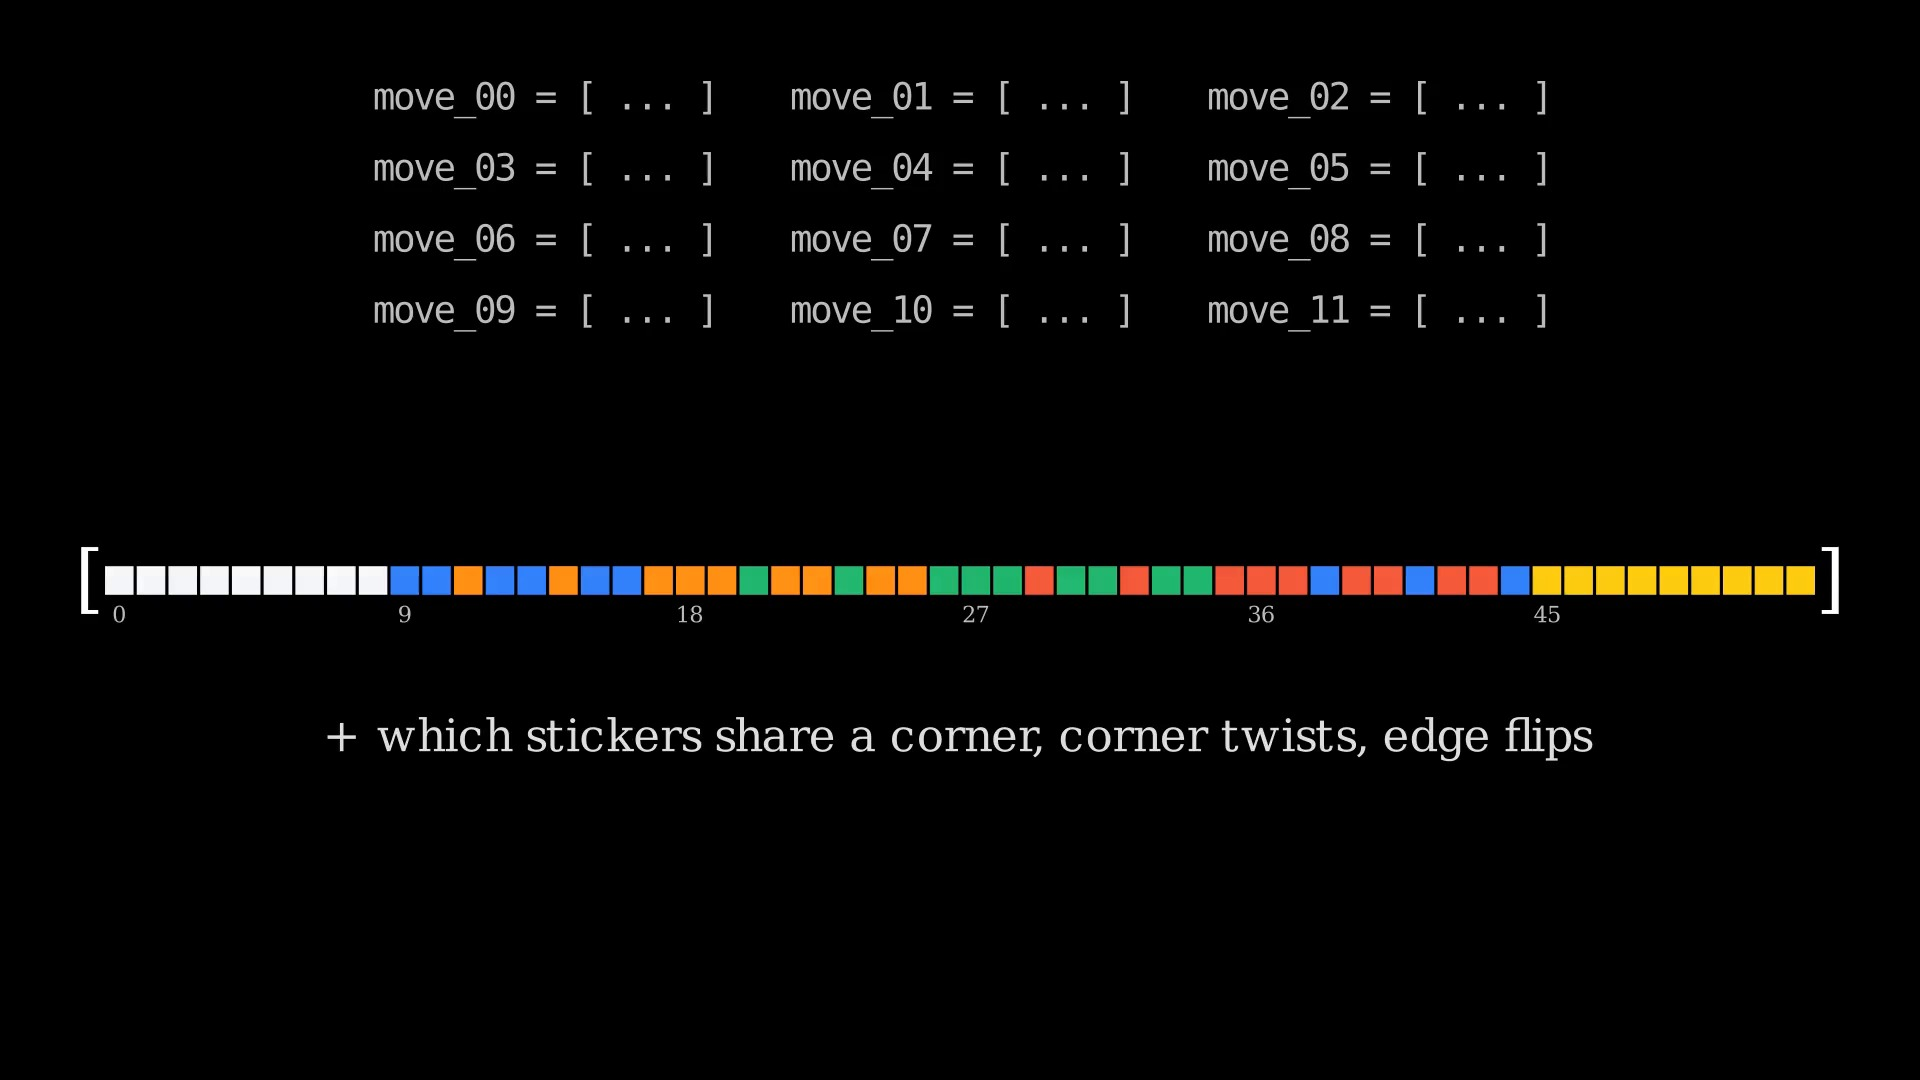
\includegraphics[width=0.90\textwidth]{figures/fig_01_permutation_tables.jpg}
\caption{用 54 张贴纸的线性列表表示魔方：12 张走法置换表，外加共角、扭转与翻转等簿记\vtag}
\label{fig:perm}
\end{figure}
\srcnote{00:00:26--00:00:40}
\end{minipage}

讲者想给出另一种写法：整个魔方的状态、每一步转动，以及“是否已经复原”的判定，都只使用向量、矩阵和点积。这个模型叫做 Eigencube。讲者展示了项目页：程序名为 \texttt{eigencube.py}，连求解器在内不足 400 行 Python，并且完全没有查找表，代码在 \url{https://github.com/smolkaj/eigencube}。

\noindent\begin{minipage}{\textwidth}
\begin{figure}[H]
\centering
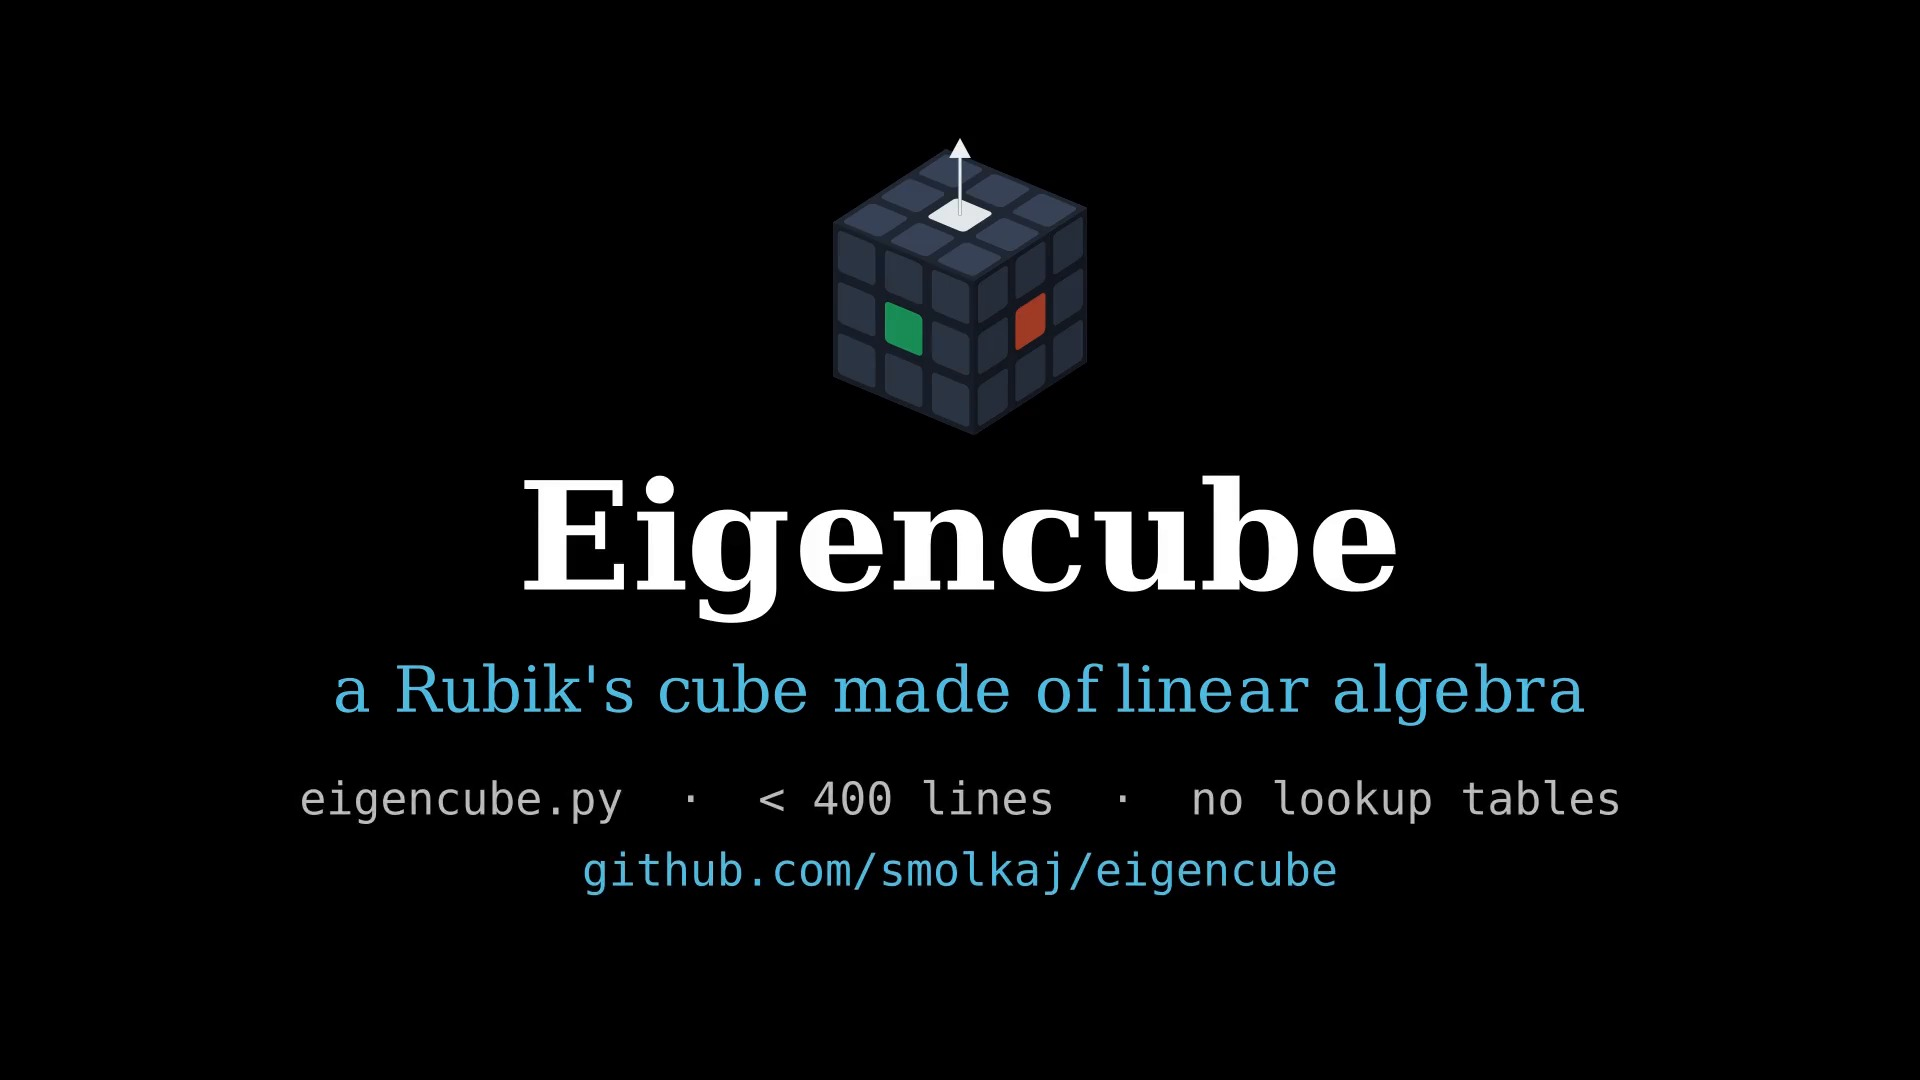
\includegraphics[width=0.90\textwidth]{figures/fig_02_eigencube_title.jpg}
\caption{Eigencube 项目页：用线性代数实现魔方，不足 400 行 Python，无查找表\vtag}
\label{fig:title}
\end{figure}
\srcnote{00:00:42--00:00:58}
\end{minipage}

\begin{knowledgebox}{本讲与《线性代数的本质》的关系}
讲者声明，整个项目长自 3Blue1Brown（Grant Sanderson）的系列视频 \emph{Essence of Linear Algebra}（线性代数的本质）。后文会调用其中关于向量、矩阵、旋转与点积的想法；若要追问“为什么矩阵乘法就是旋转后的向量”，讲者把详细解释指向该系列，而不是在本讲里重推一遍。
\end{knowledgebox}

\subsection{本章小结}

把贴纸排成列表，表面上记下了全部颜色，却把一次转动变成 12 张置换表和一堆额外簿记，几何关系被抹掉。Eigencube 的目标是：让状态、走法与复原判定都回到向量和矩阵上。为此，需要先借用线性代数里描述旋转的语言。

\section{向量、矩阵与特征向量：后面要用的语言}

先看一张带网格的平面。向量是从原点出发的箭头，用坐标来写。讲者举的例子是“二、一”：向右走两步，再向上走一步。这两步分别由两个特殊向量量出：绿色的 $\mathbf{e}_x$ 是向右的一步，红色的 $\mathbf{e}_y$ 是向上的一步，合称一组基。\emph{Essence of Linear Algebra} 把它们叫做 i-hat 与 j-hat。平面上每一个向量都是它们的组合；这个例子便是
\[
\vec{u}=2\mathbf{e}_x+1\mathbf{e}_y.
\]
\begin{itemize}
\item $\vec{u}$：从原点出发的示例向量，坐标为 $\begin{bmatrix}2\\1\end{bmatrix}$。
\item $\mathbf{e}_x$、$\mathbf{e}_y$：向右、向上的单位基向量。
\end{itemize}

\noindent\begin{minipage}{\textwidth}
\begin{figure}[H]
\centering
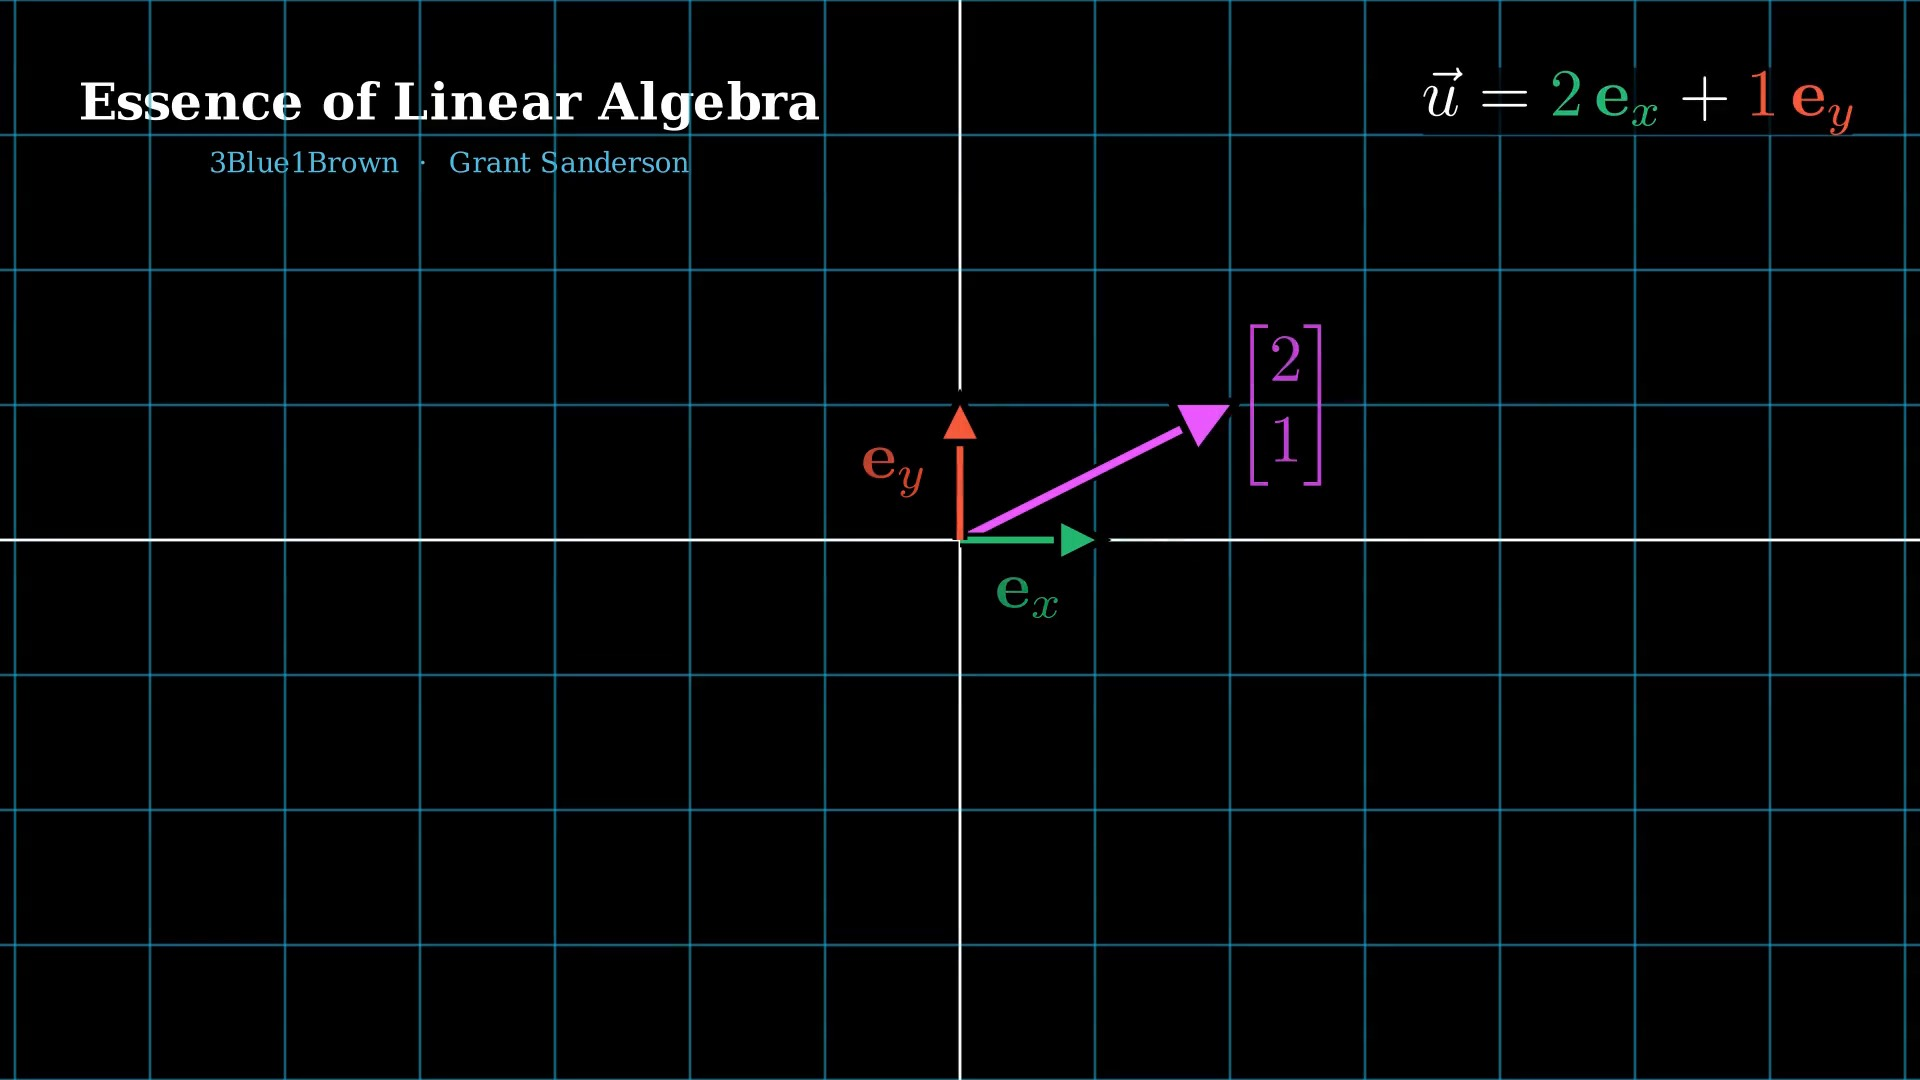
\includegraphics[width=0.90\textwidth]{figures/fig_03_vector_basis.jpg}
\caption{平面上的基与示例向量：$\vec{u}=2\mathbf{e}_x+1\mathbf{e}_y$，坐标为 $[2,1]^{\mathrm{T}}$\vtag}
\label{fig:basis}
\end{figure}
\srcnote{00:01:37--00:01:52}
\end{minipage}

矩阵被讲者说成“变换整个空间的一种方式”。把整个平面绕原点逆时针转四分之一圈后，$\mathbf{e}_x$ 落到 $(0,1)$，$\mathbf{e}_y$ 落到 $(-1,0)$。把这两个落点并排写成列，就得到这次旋转的矩阵
\[
R=\begin{bmatrix}0&-1\\1&0\end{bmatrix}.
\]
\begin{itemize}
\item $R$ 的第一列是 $\mathbf{e}_x$ 转过之后的位置 $(0,1)$。
\item $R$ 的第二列是 $\mathbf{e}_y$ 转过之后的位置 $(-1,0)$。
\end{itemize}
原来的 $\vec{u}$ 仍然是“两步 $\mathbf{e}_x$ 加一步 $\mathbf{e}_y$”，只是这两步已经换成了移动后的基。用矩阵乘向量算出来，就是
\[
R\begin{bmatrix}2\\1\end{bmatrix}
=2\begin{bmatrix}0\\1\end{bmatrix}
+1\begin{bmatrix}-1\\0\end{bmatrix}
=\begin{bmatrix}-1\\2\end{bmatrix}.
\]
\begin{itemize}
\item 左侧是对原坐标做矩阵乘法。
\item 右侧是用移动后的基重新组合同一个系数 $2$ 与 $1$，得到旋转后的向量 $(-1,2)$。
\end{itemize}

\noindent\begin{minipage}{\textwidth}
\begin{figure}[H]
\centering
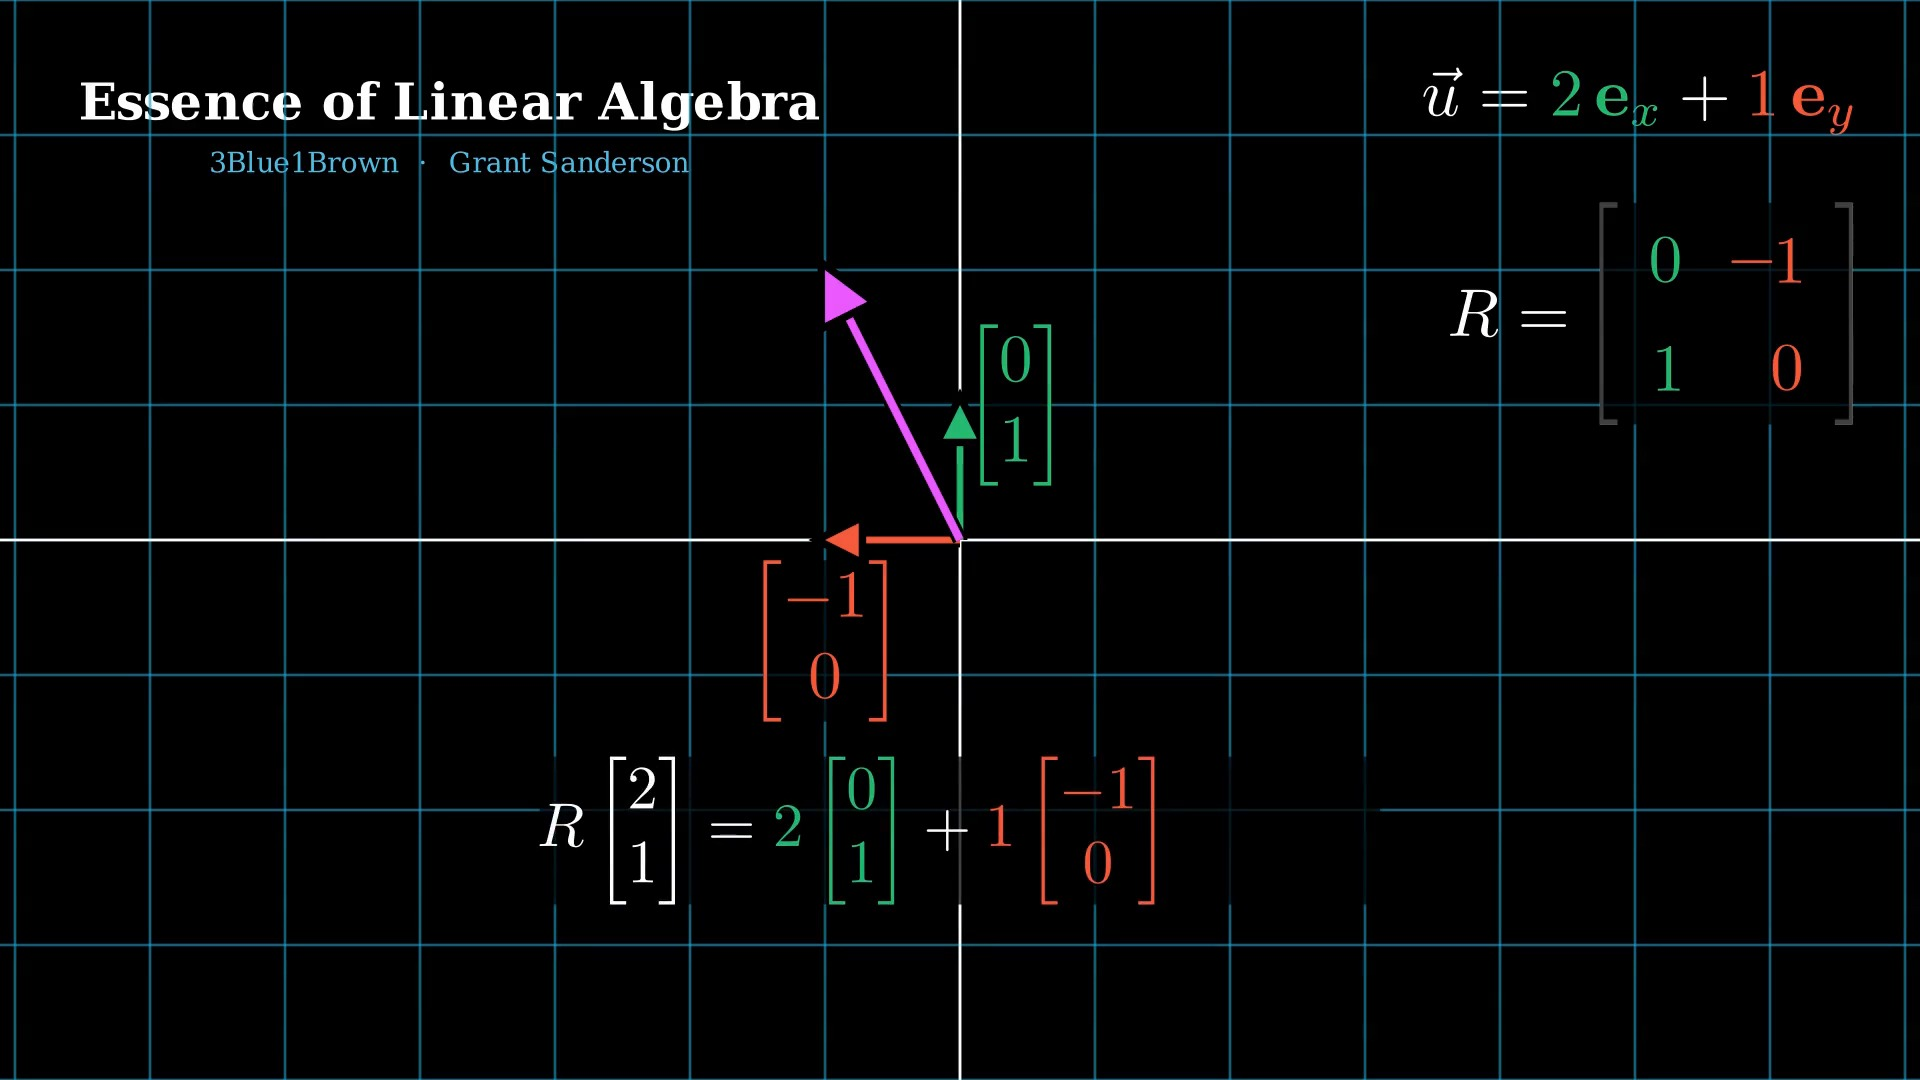
\includegraphics[width=0.90\textwidth]{figures/fig_04_rotation_matrix.jpg}
\caption{绕原点逆时针四分之一转：用基向量落点写出 $R$，并得到 $R[2,1]^{\mathrm{T}}=[-1,2]^{\mathrm{T}}$\vtag}
\label{fig:R2d}
\end{figure}
\srcnote{00:02:08--00:02:26}
\end{minipage}

\begin{importantbox}{贯穿后文的规则}
绕原点的旋转就是一个矩阵 $R$；用这个矩阵去乘一个向量，得到的就是旋转后的向量：$R\vec{u}=\vec{u}'$。后文把这条规则直接搬到三维。
\end{importantbox}

最后还要一个词。如果一次变换把某个向量留在原地，这个向量就叫做特征向量，对应的特征值是 $1$。平面上的四分之一转不会留下任何箭头；但到了三维，每次旋转都有一根这样的轴。讲者请观众先记住这一点。

\noindent\begin{minipage}{\textwidth}
\begin{figure}[H]
\centering
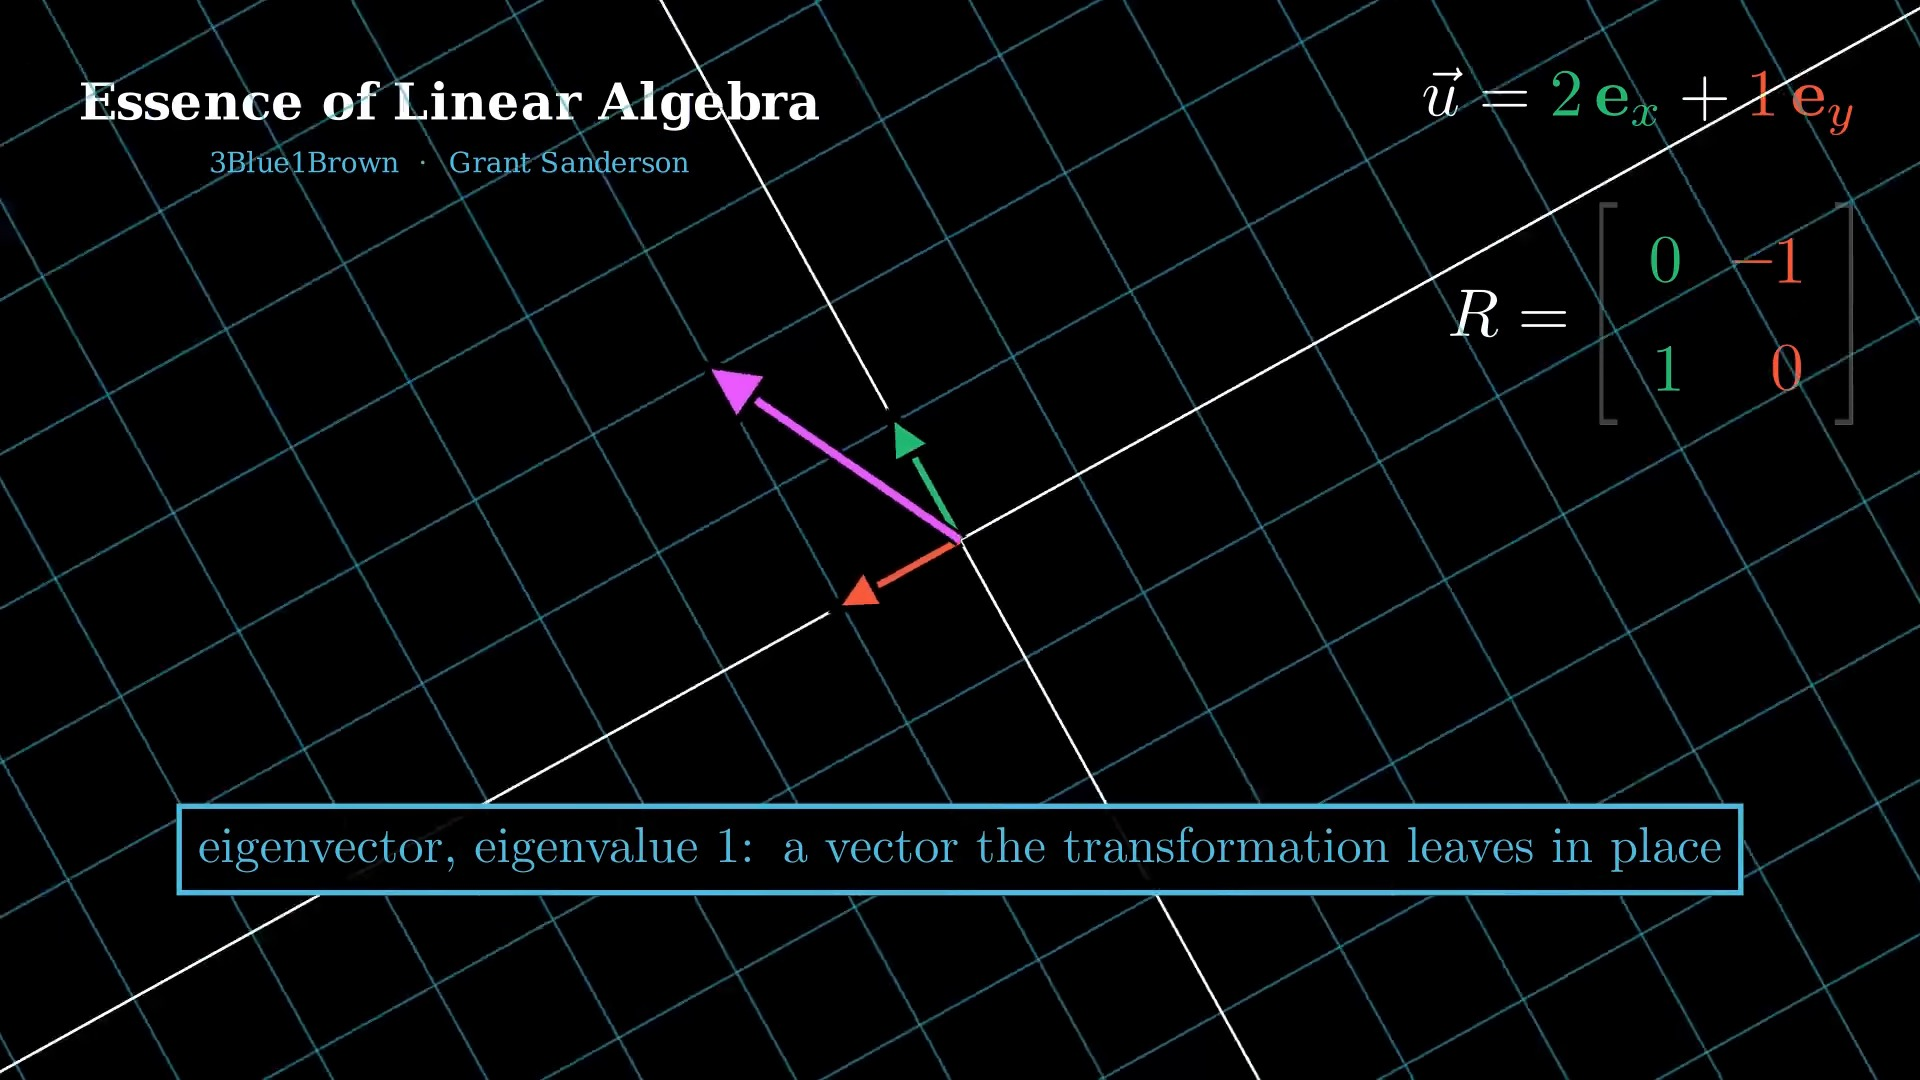
\includegraphics[width=0.90\textwidth]{figures/fig_05_eigenvector.jpg}
\caption{特征值 $1$ 的特征向量：变换之后仍然留在原处的向量。平面四分之一转没有这样的箭头\vtag}
\label{fig:eigen}
\end{figure}
\srcnote{00:02:42--00:03:00}
\end{minipage}

\subsection{本章小结}

向量由基组合而成，旋转矩阵的列就是基的落点，矩阵乘向量给出旋转后的结果。三维里，旋转轴是特征值 $1$ 的特征向量。下一步要把这套语言安到魔方内部那根永不移动的十字上。

\section{固定的芯轴：给每个小立方块一个地址}

把实体魔方拆开，会看到它的骨架：一个坚实的三维十字，芯在中央，六个中心块固定在六条臂上。关键观察是：每一次走法都是让某一个外面绕十字的一条臂转动。中心块会在原地自旋，但从不离开原位。这根十字是永久固定的。

用上一节的话说，绕某条臂转动时，这条臂恰好留在原地，因此它是这些转动的特征向量。讲者指出，Eigencube 的名字就来自这里。

\begin{importantbox}{名称从何而来}
“某种永不移动的东西”正是建立坐标系所需要的参照。十字的臂是绕它转动时的特征向量，模型由此得名 Eigencube。
\end{importantbox}

于是把原点放在芯上，让十字的臂成为坐标轴：$x$ 指向前方，$y$ 指向右方，$z$ 指向上方。每条轴都贯穿到对面的中心。每个小立方块因此得到一个地址：从芯指向该块中心的向量 $c$。

\noindent\begin{minipage}{\textwidth}
\begin{figure}[H]
\centering
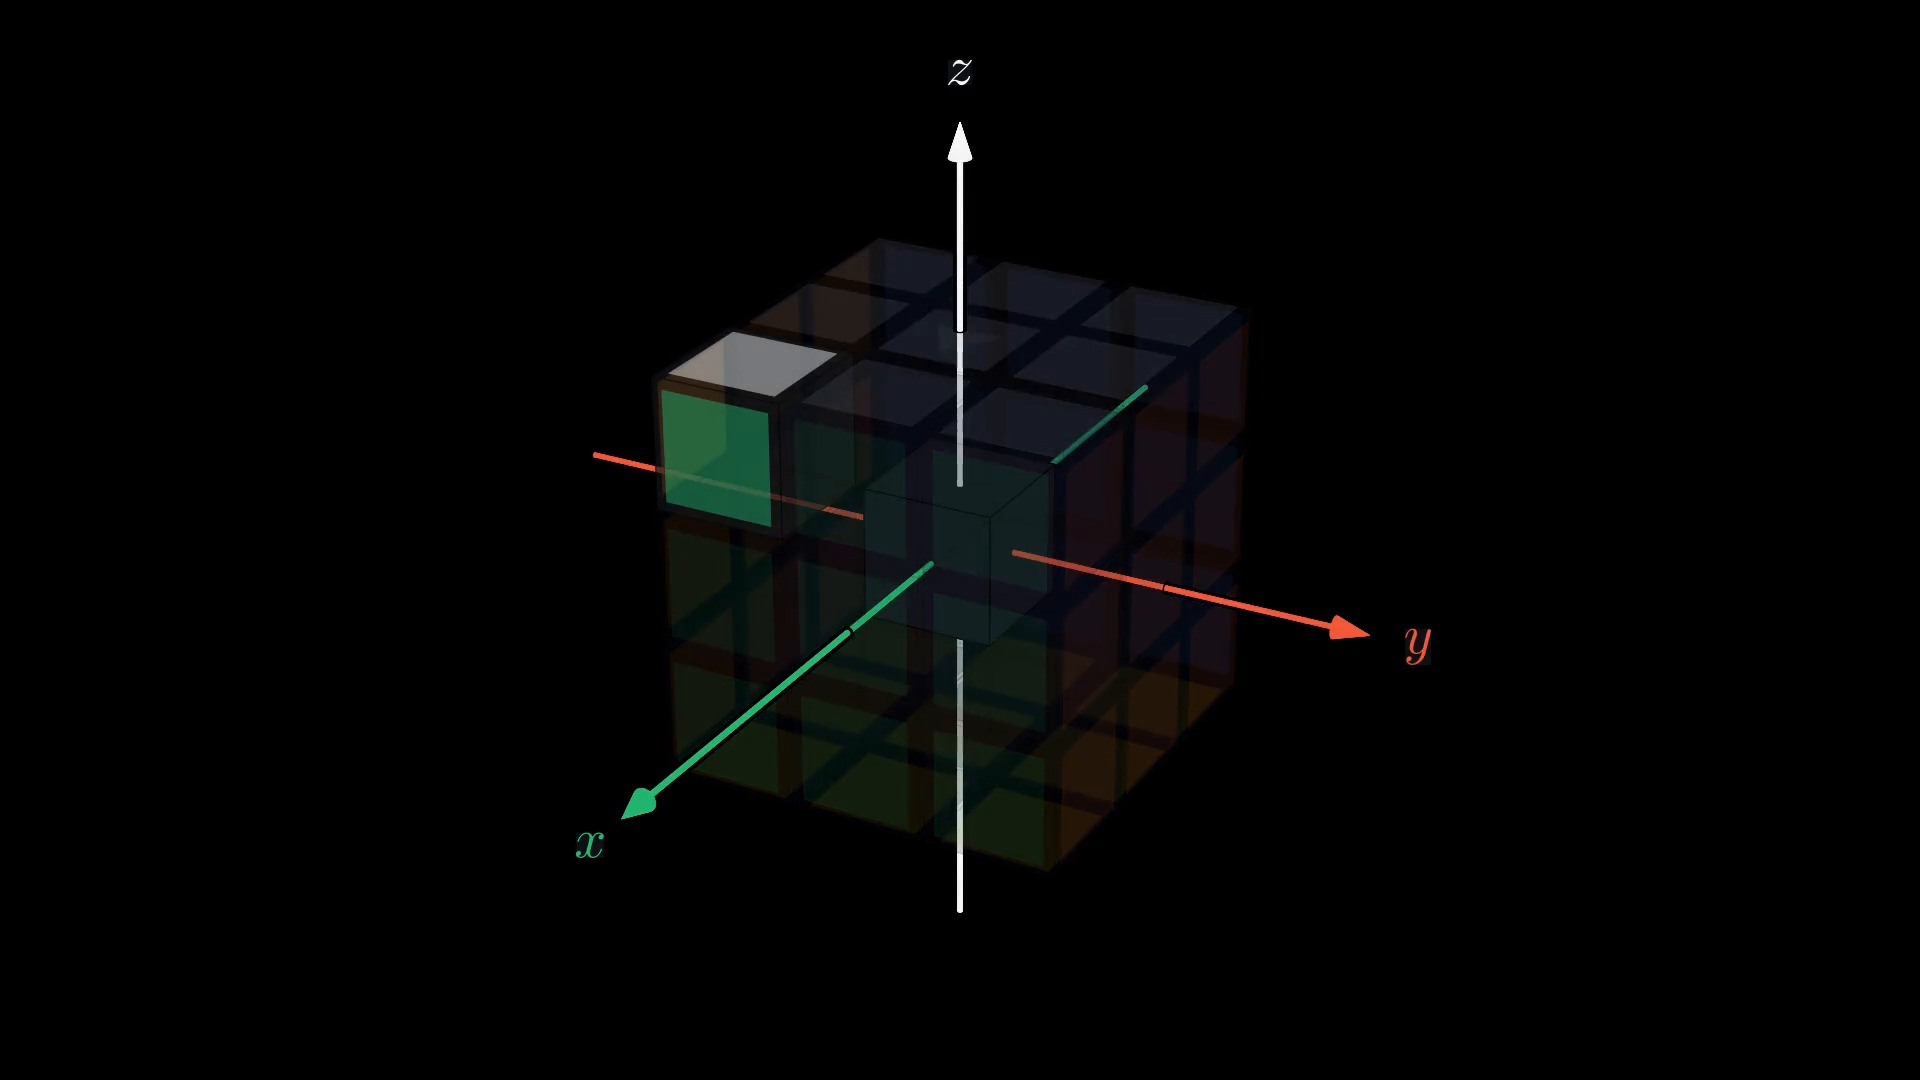
\includegraphics[width=0.90\textwidth]{figures/fig_06_axes.jpg}
\caption{以芯为原点、以十字的臂为轴：$x$ 朝前，$y$ 朝右，$z$ 朝上\vtag}
\label{fig:axes}
\end{figure}
\srcnote{00:03:49--00:04:04}
\end{minipage}

以讲者指出的那个角块为例：向前一步、向左一步、再向上一步，于是
\[
c=(1,-1,1),\qquad c\in\{-1,0,1\}^3.
\]
\begin{itemize}
\item $c$：从小立方块中心指向其家乡位置的地址向量。
\item 每个坐标只能取 $-1$、$0$ 或 $1$。
\end{itemize}
一个中心的例子是 $(0,1,0)$，一条棱的例子是 $(0,1,1)$。

\noindent\begin{minipage}{\textwidth}
\begin{figure}[H]
\centering
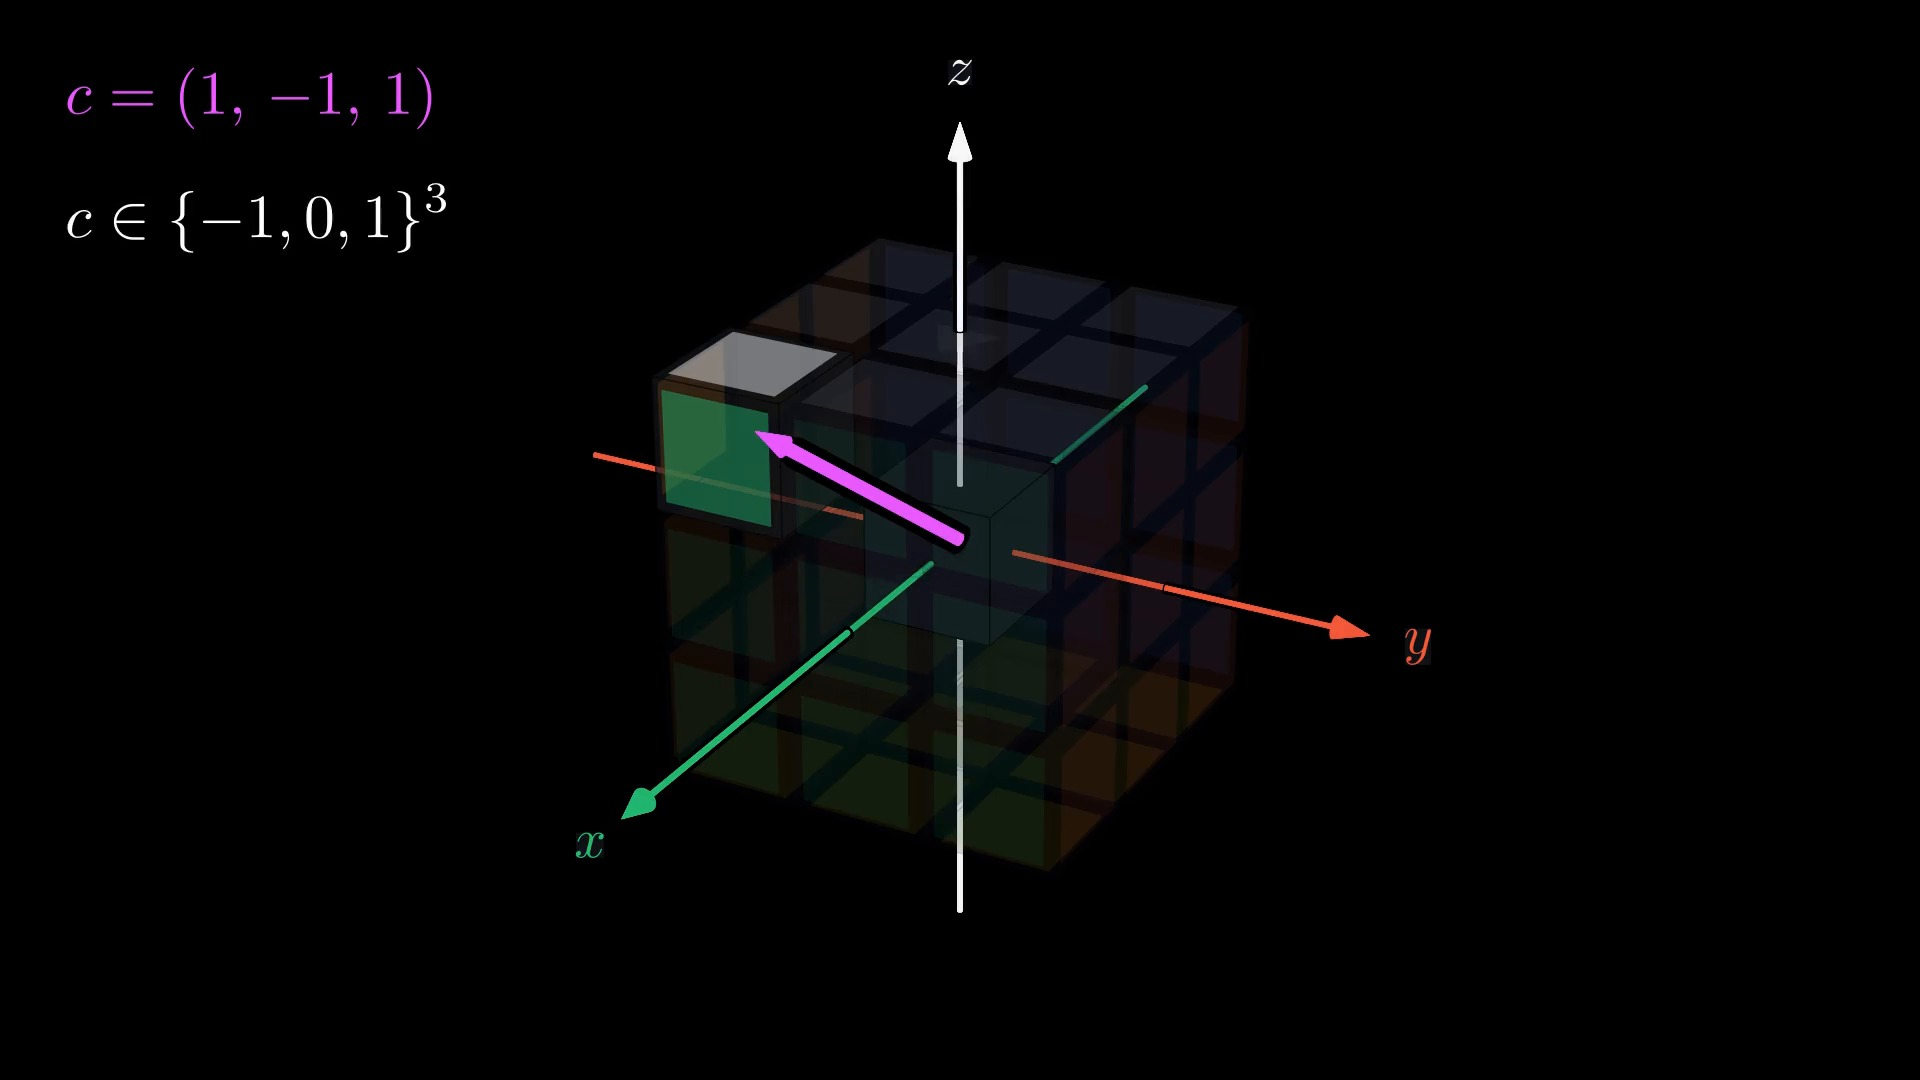
\includegraphics[width=0.90\textwidth]{figures/fig_07_cubelet_address.jpg}
\caption{前左上角块的地址 $c=(1,-1,1)$，全体小立方块的坐标都属于 $\{-1,0,1\}^3$\vtag}
\label{fig:addr}
\end{figure}
\srcnote{00:04:04--00:04:28}
\end{minipage}

这套坐标是否好用，沿 $x$ 轴看一眼就能感觉到。魔方被分成三层：$x=1$ 在前，$x=0$ 在中，$x=-1$ 在后。中间那一层的小立方块满足 $x=0$，沿 $x$ 方向“藏在里面”，前后都没有贴纸；外层的小立方块则在该侧露出一张贴纸。因此 $|x|$ 是一个开关：这块是否沿 $x$ 轴露出贴纸。$y$ 与 $z$ 同理。

\noindent\begin{minipage}{\textwidth}
\begin{figure}[H]
\centering
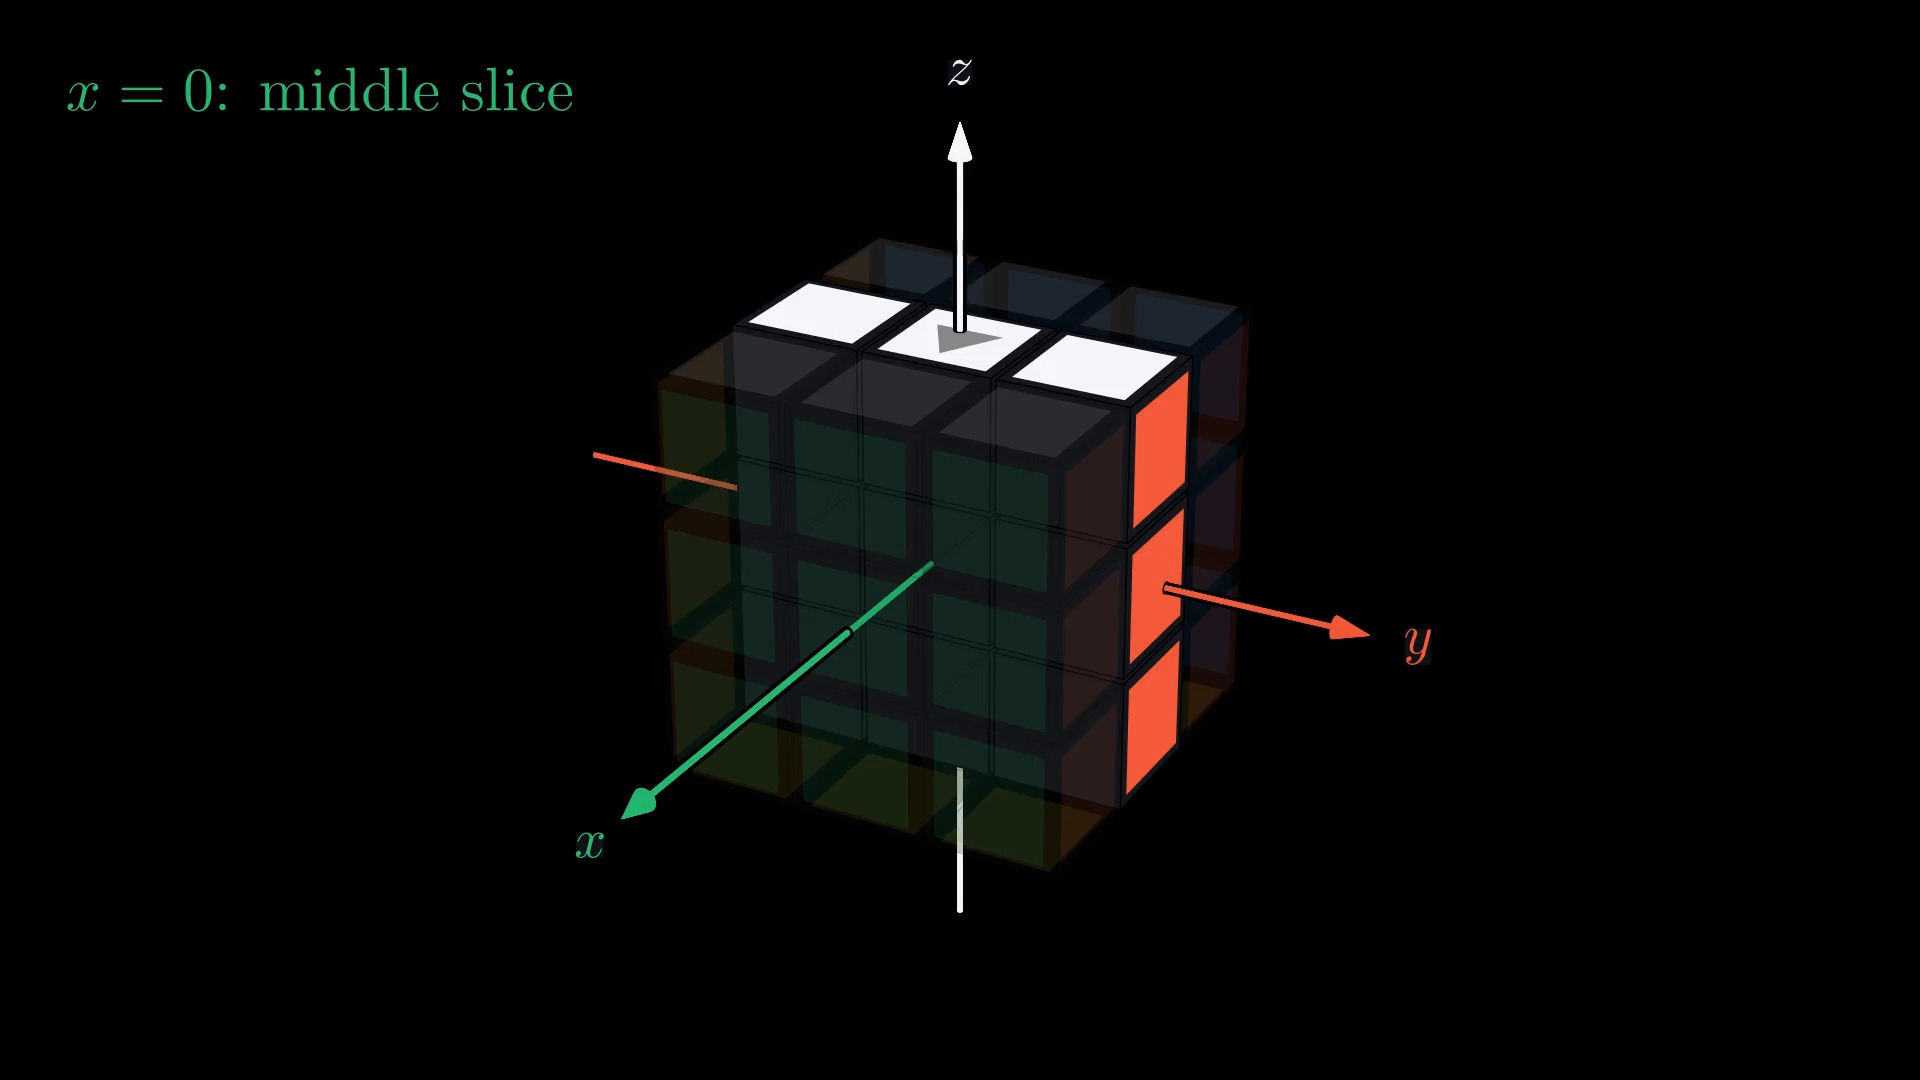
\includegraphics[width=0.90\textwidth]{figures/fig_08_middle_slice.jpg}
\caption{$x=0$ 的中间层：沿 $x$ 方向不朝前或朝后露出贴纸\vtag}
\label{fig:slice}
\end{figure}
\srcnote{00:04:36--00:05:07}
\end{minipage}

\subsection{本章小结}

固定的十字提供了原点与坐标轴，每个小立方块都有地址 $c\in\{-1,0,1\}^3$。坐标的绝对值还直接告诉你，这块是否在某个方向露出贴纸。把三个开关加起来，就得到下节的贴纸计数。

\section{曼哈顿范数怎样数出贴纸}

把 $|x|$、$|y|$、$|z|$ 加起来，得到 $c$ 的曼哈顿范数，它恰好等于这块上的贴纸数：
\[
\|c\|_1=|x|+|y|+|z|=\text{贴纸数}.
\]
\begin{itemize}
\item $\|c\|_1$：$c$ 三个坐标绝对值之和。
\item 其数值等于该小立方块露出的贴纸张数。
\end{itemize}

按这个范数分类，全部零件会被自动分开：隐藏的芯是 $(0,0,0)$，范数为 $0$，共 $1$ 个；中心如 $(0,0,1)$，范数为 $1$，共 $6$ 个；棱如 $(1,0,1)$，范数为 $2$，共 $12$ 条；角如 $(1,1,1)$，范数为 $3$，共 $8$ 个。于是
\[
1+6+12+8=27.
\]
讲者强调，这是全部 27 个零件，只靠一次求和就按类型排好，不必另做分类器。注意这里把看不见的芯也算进去，因此是 27 而不是开场提到的 26 个可见塑料块。

\begin{table}[H]
\centering
\begin{tabular}{lccc}
\toprule
类型 & 示例坐标 & 曼哈顿范数（贴纸数） & 个数 \\
\midrule
芯 & $(0,0,0)$ & $0$ & $1$ \\
中心 & $(0,0,1)$ & $1$ & $6$ \\
棱 & $(1,0,1)$ & $2$ & $12$ \\
角 & $(1,1,1)$ & $3$ & $8$ \\
\midrule
合计 & & & $27$ \\
\bottomrule
\end{tabular}
\caption{用 $\|c\|_1$ 按类型清点全部零件}
\end{table}

\noindent\begin{minipage}{\textwidth}
\begin{figure}[H]
\centering
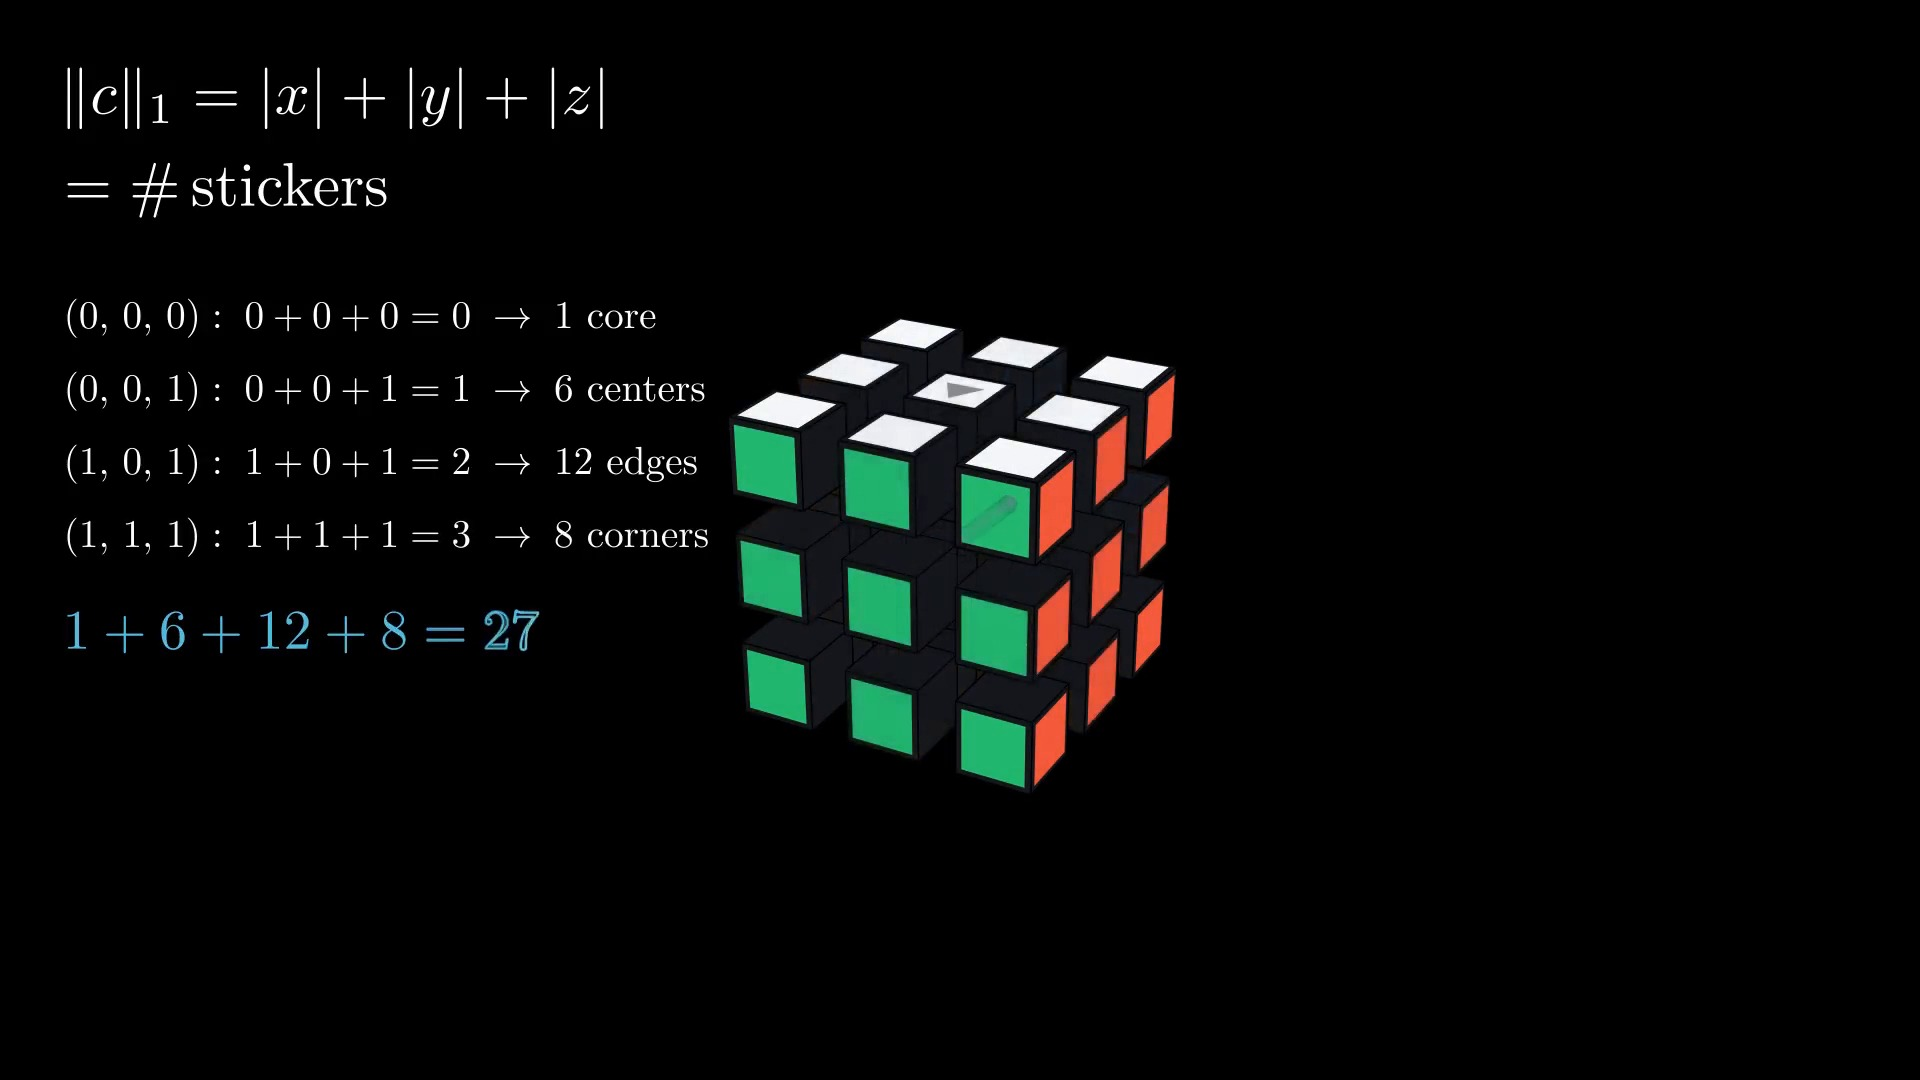
\includegraphics[width=0.90\textwidth]{figures/fig_09_manhattan_norm.jpg}
\caption{曼哈顿范数等于贴纸数，并给出 $1+6+12+8=27$ 的分类清点\vtag}
\label{fig:norm}
\end{figure}
\srcnote{00:05:15--00:05:42}
\end{minipage}

\subsection{本章小结}

$\|c\|_1$ 既是坐标的绝对值之和，也是贴纸张数，还把芯、中心、棱、角四种零件一次分开。接下来的问题是：这些贴纸上的颜色，要不要另外发明一套名字？

\section{颜色就是基向量，diag$(c)$ 同时记下朝向与颜色}

程序里也许会用字符串或枚举来表示颜色。但再看那些中心：它们永不移动，并且各自决定了复原时那一面应有的颜色。绿色中心始终在 $(1,0,0)$，也就是沿 $x$ 的一步；红色中心在 $(0,1,0)$；白色中心在 $(0,0,1)$。这三个向量正是标准基 $\mathbf{e}_x$、$\mathbf{e}_y$、$\mathbf{e}_z$——与平面回顾中的基相同，只是多了第三维。

\begin{importantbox}{不必为颜色另起名字}
讲者的做法是：一种颜色就是一个单位向量。绿是 $\mathbf{e}_x$，红是 $\mathbf{e}_y$，白是 $\mathbf{e}_z$；蓝、橙、黄则是它们的相反方向 $-\mathbf{e}_x$、$-\mathbf{e}_y$、$-\mathbf{e}_z$。
\end{importantbox}

\noindent\begin{minipage}{\textwidth}
\begin{figure}[H]
\centering
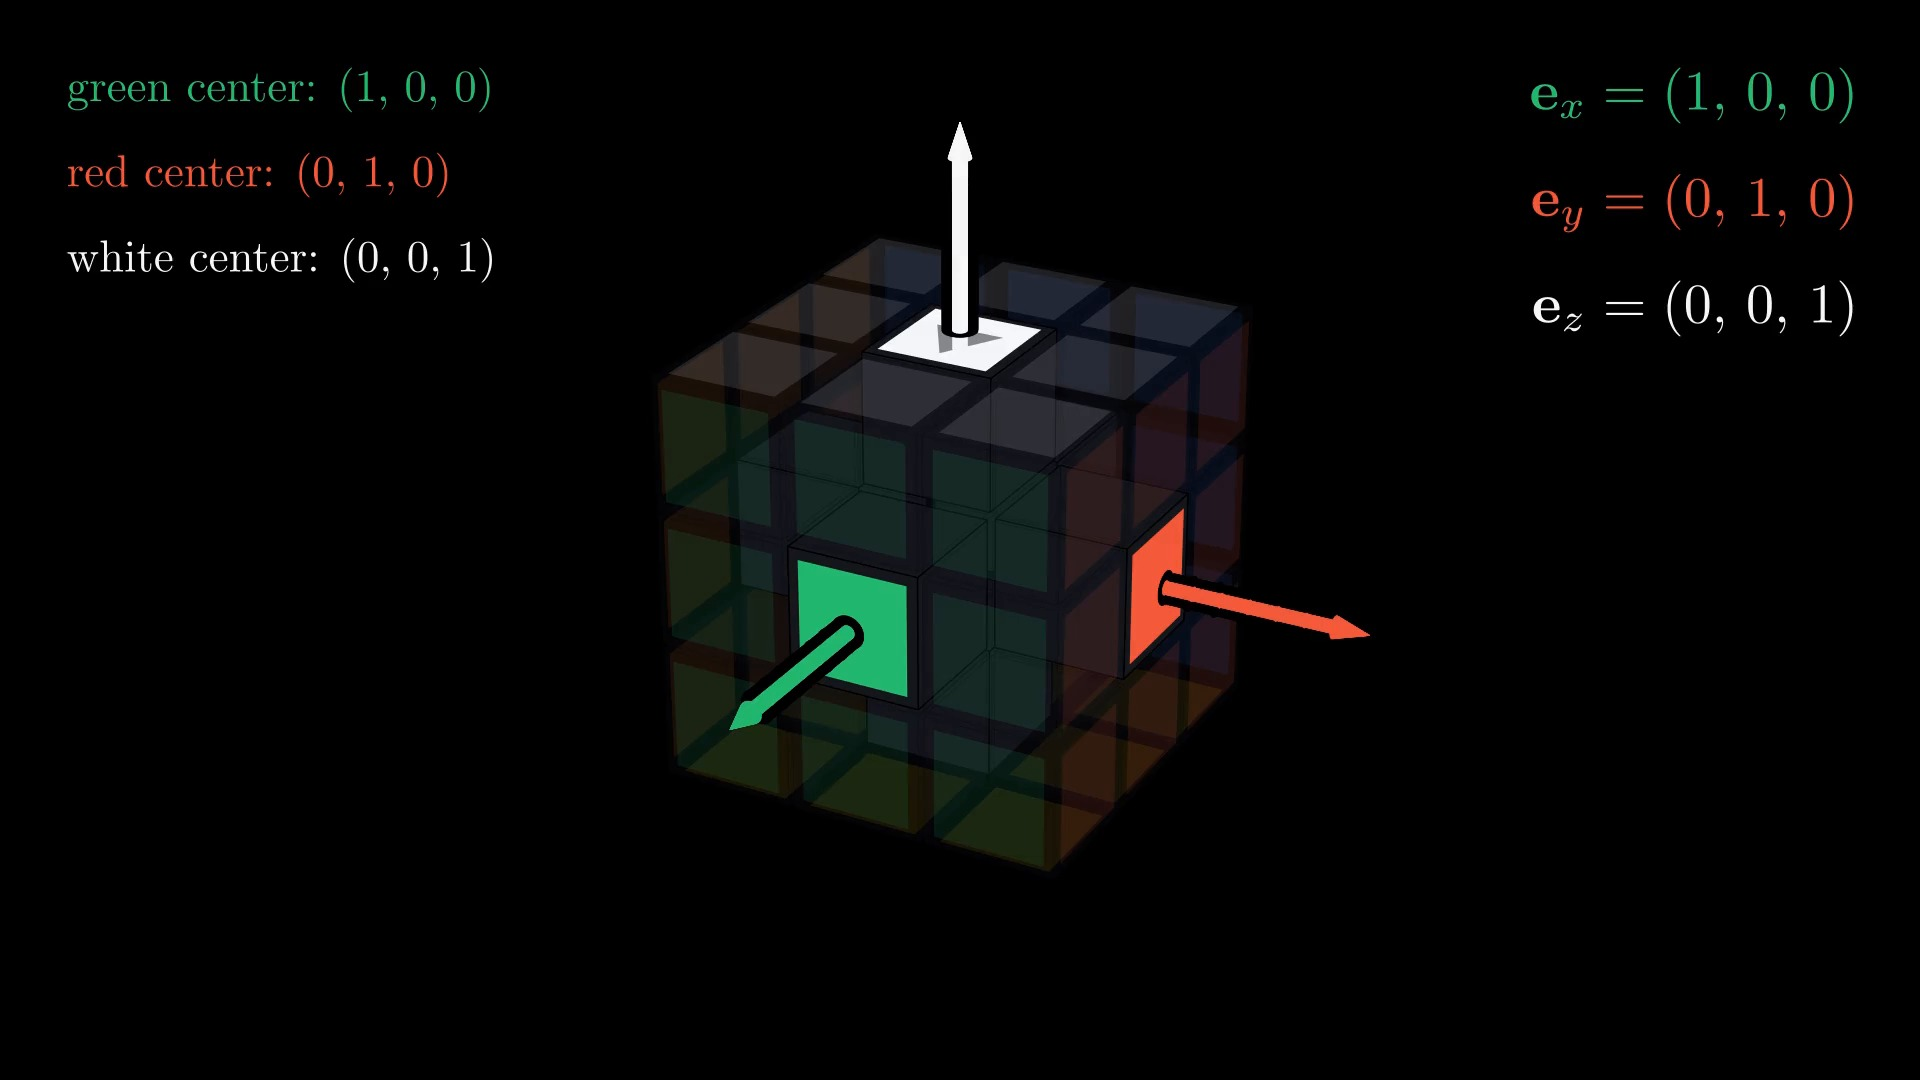
\includegraphics[width=0.90\textwidth]{figures/fig_10_colors_basis.jpg}
\caption{三个可见中心与标准基重合：绿 $\mathbf{e}_x=(1,0,0)$，红 $\mathbf{e}_y=(0,1,0)$，白 $\mathbf{e}_z=(0,0,1)$\vtag}
\label{fig:colors}
\end{figure}
\srcnote{00:06:03--00:06:27}
\end{minipage}

蓝、橙、黄朝向观众的背面。把视角转到后方，就可以看到它们各自沿着与配对颜色相反的方向指出。

\noindent\begin{minipage}{\textwidth}
\begin{figure}[H]
\centering
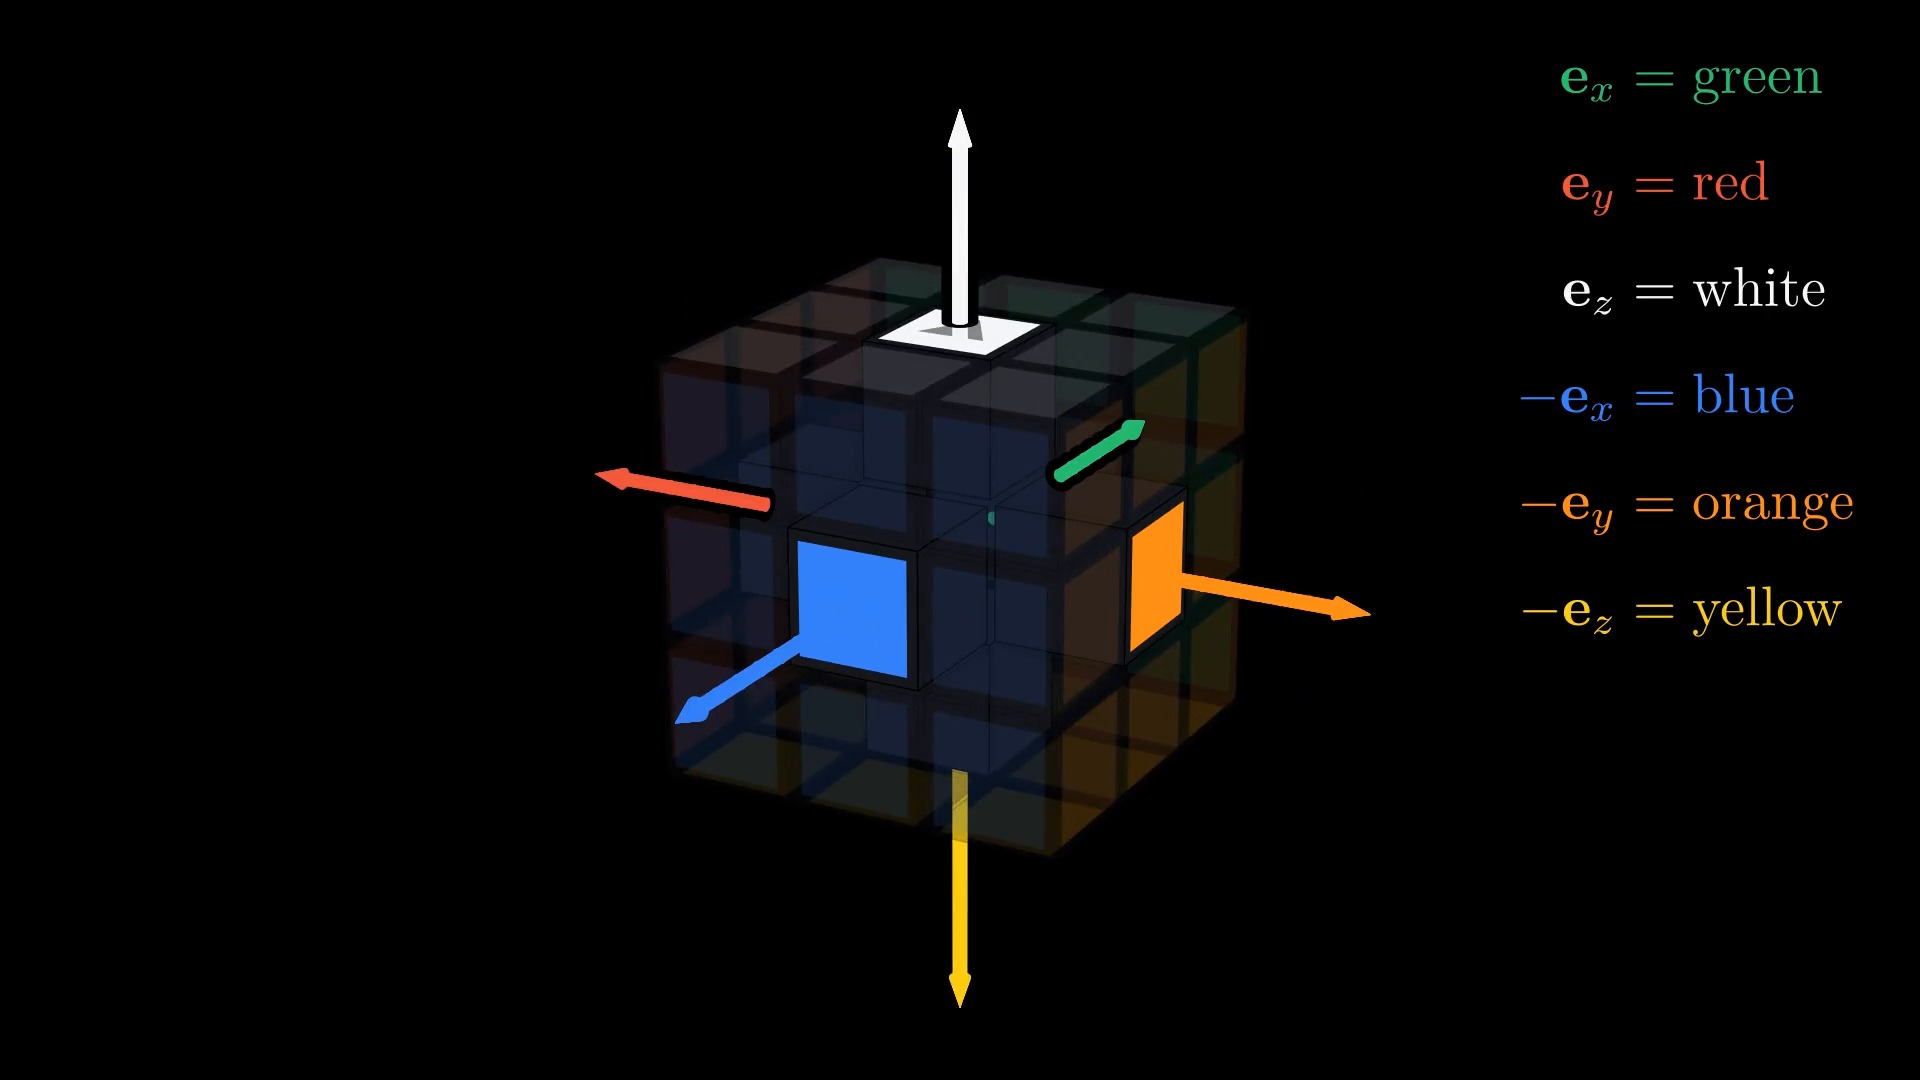
\includegraphics[width=0.90\textwidth]{figures/fig_11_opposite_colors.jpg}
\caption{从背面观察：蓝、橙、黄分别是 $-\mathbf{e}_x$、$-\mathbf{e}_y$、$-\mathbf{e}_z$\vtag}
\label{fig:opp}
\end{figure}
\srcnote{00:06:36--00:06:57}
\end{minipage}

讲者称之为自己“最喜欢的技巧”。取前、右、上那个角块，地址为 $c=(1,1,1)$，把它沿三个轴拆开：
\[
c=1\mathbf{e}_x+1\mathbf{e}_y+1\mathbf{e}_z.
\]
从这块自身画出这三条箭头，每一条都正好穿过一块贴纸；又因为颜色就是基向量，箭头同时也是那张贴纸的颜色：绿在前，红在右，白在上。把这三条箭头并排写成矩阵的列，就得到以 $c$ 为对角线的对角矩阵 $\mathrm{diag}(c)$：
\[
\mathrm{diag}(c)=\begin{bmatrix}1&0&0\\0&1&0\\0&0&1\end{bmatrix}.
\]
\begin{itemize}
\item 第一列是 $\mathbf{e}_x$，也就是绿色、朝前的贴纸。
\item 第二列是 $\mathbf{e}_y$，红色、朝右。
\item 第三列是 $\mathbf{e}_z$，白色、朝上。
\end{itemize}
每一列既给出贴纸朝哪，也给出它是什么颜色。

\noindent\begin{minipage}{\textwidth}
\begin{figure}[H]
\centering
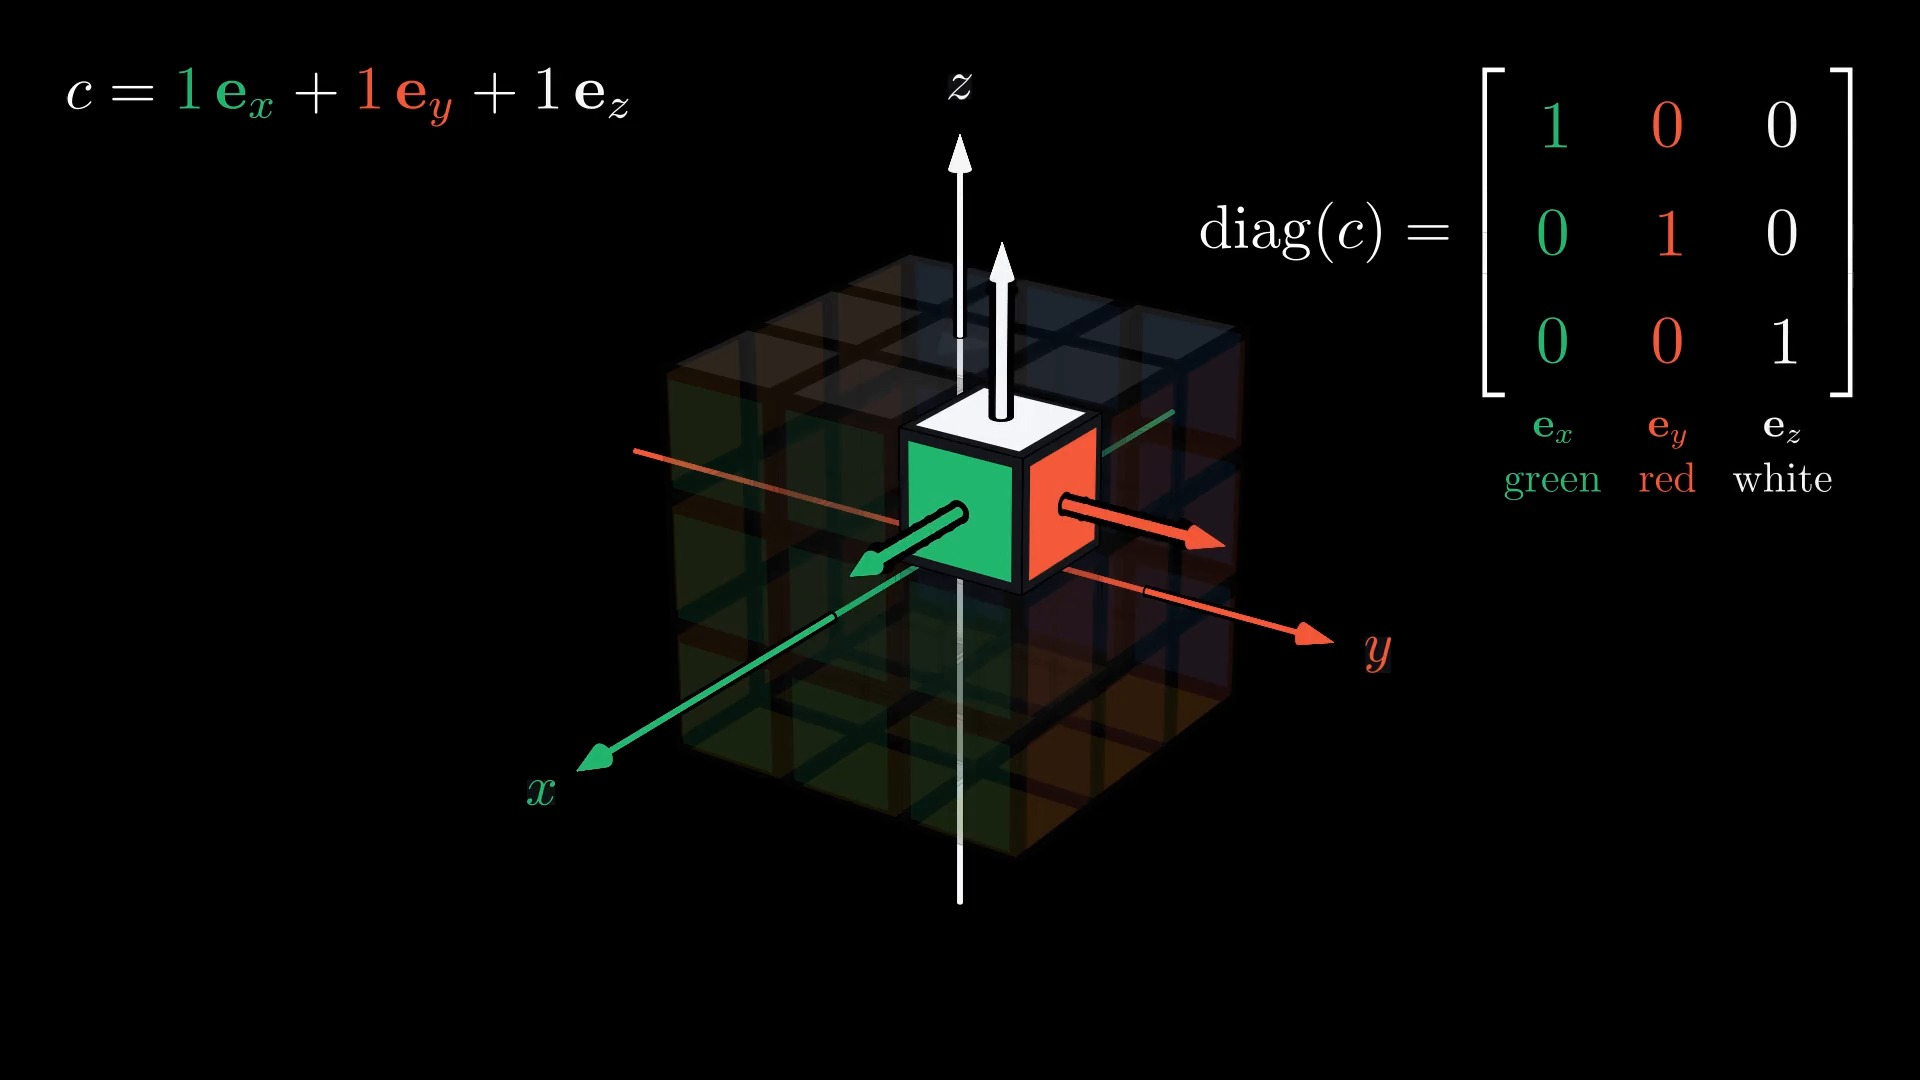
\includegraphics[width=0.90\textwidth]{figures/fig_12_diag_c_corner.jpg}
\caption{角块 $c=\mathbf{e}_x+\mathbf{e}_y+\mathbf{e}_z$：$\mathrm{diag}(c)$ 的三列依次为绿、红、白\vtag}
\label{fig:diagc}
\end{figure}
\srcnote{00:07:36--00:08:03}
\end{minipage}

再看一条棱，$c=(1,0,1)$。中间坐标为 $0$，所以中间那一列全是零：这块沿 $y$ 方向没有贴纸，矩阵里相应的贴纸就自行消失。一个中心只剩下一个非零列。于是，非零列的个数——矩阵的秩——再次等于贴纸数。

\noindent\begin{minipage}{\textwidth}
\begin{figure}[H]
\centering
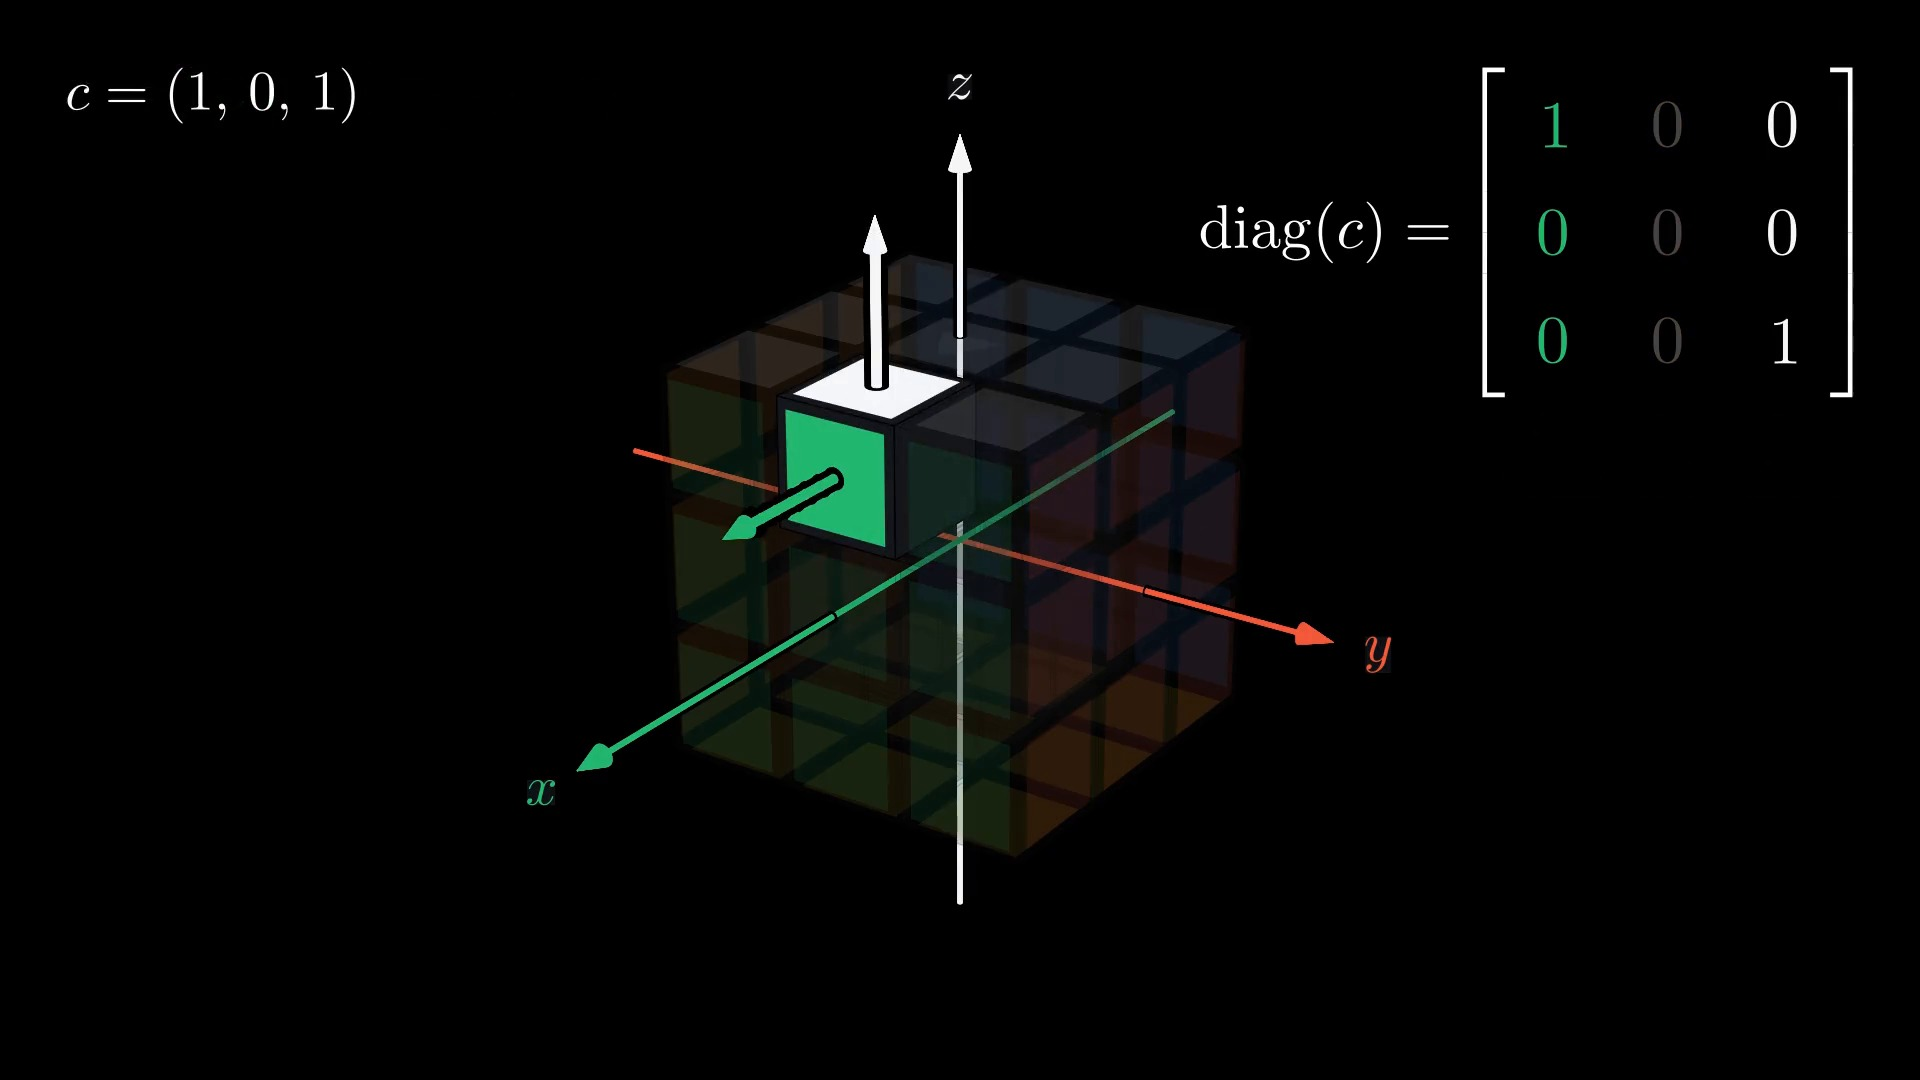
\includegraphics[width=0.90\textwidth]{figures/fig_13_diag_c_edge.jpg}
\caption{棱块 $c=(1,0,1)$：中间列全零，表示沿 $y$ 没有贴纸\vtag}
\label{fig:edge}
\end{figure}
\srcnote{00:08:03--00:08:17}
\end{minipage}

讲者把这一点收成三句话：$\mathrm{diag}(c)$ 同时告诉你，这块有多少张贴纸（它的秩）、每张朝哪（非零列）、以及每张是什么颜色（正是这些列本身）。

\noindent\begin{minipage}{\textwidth}
\begin{figure}[H]
\centering
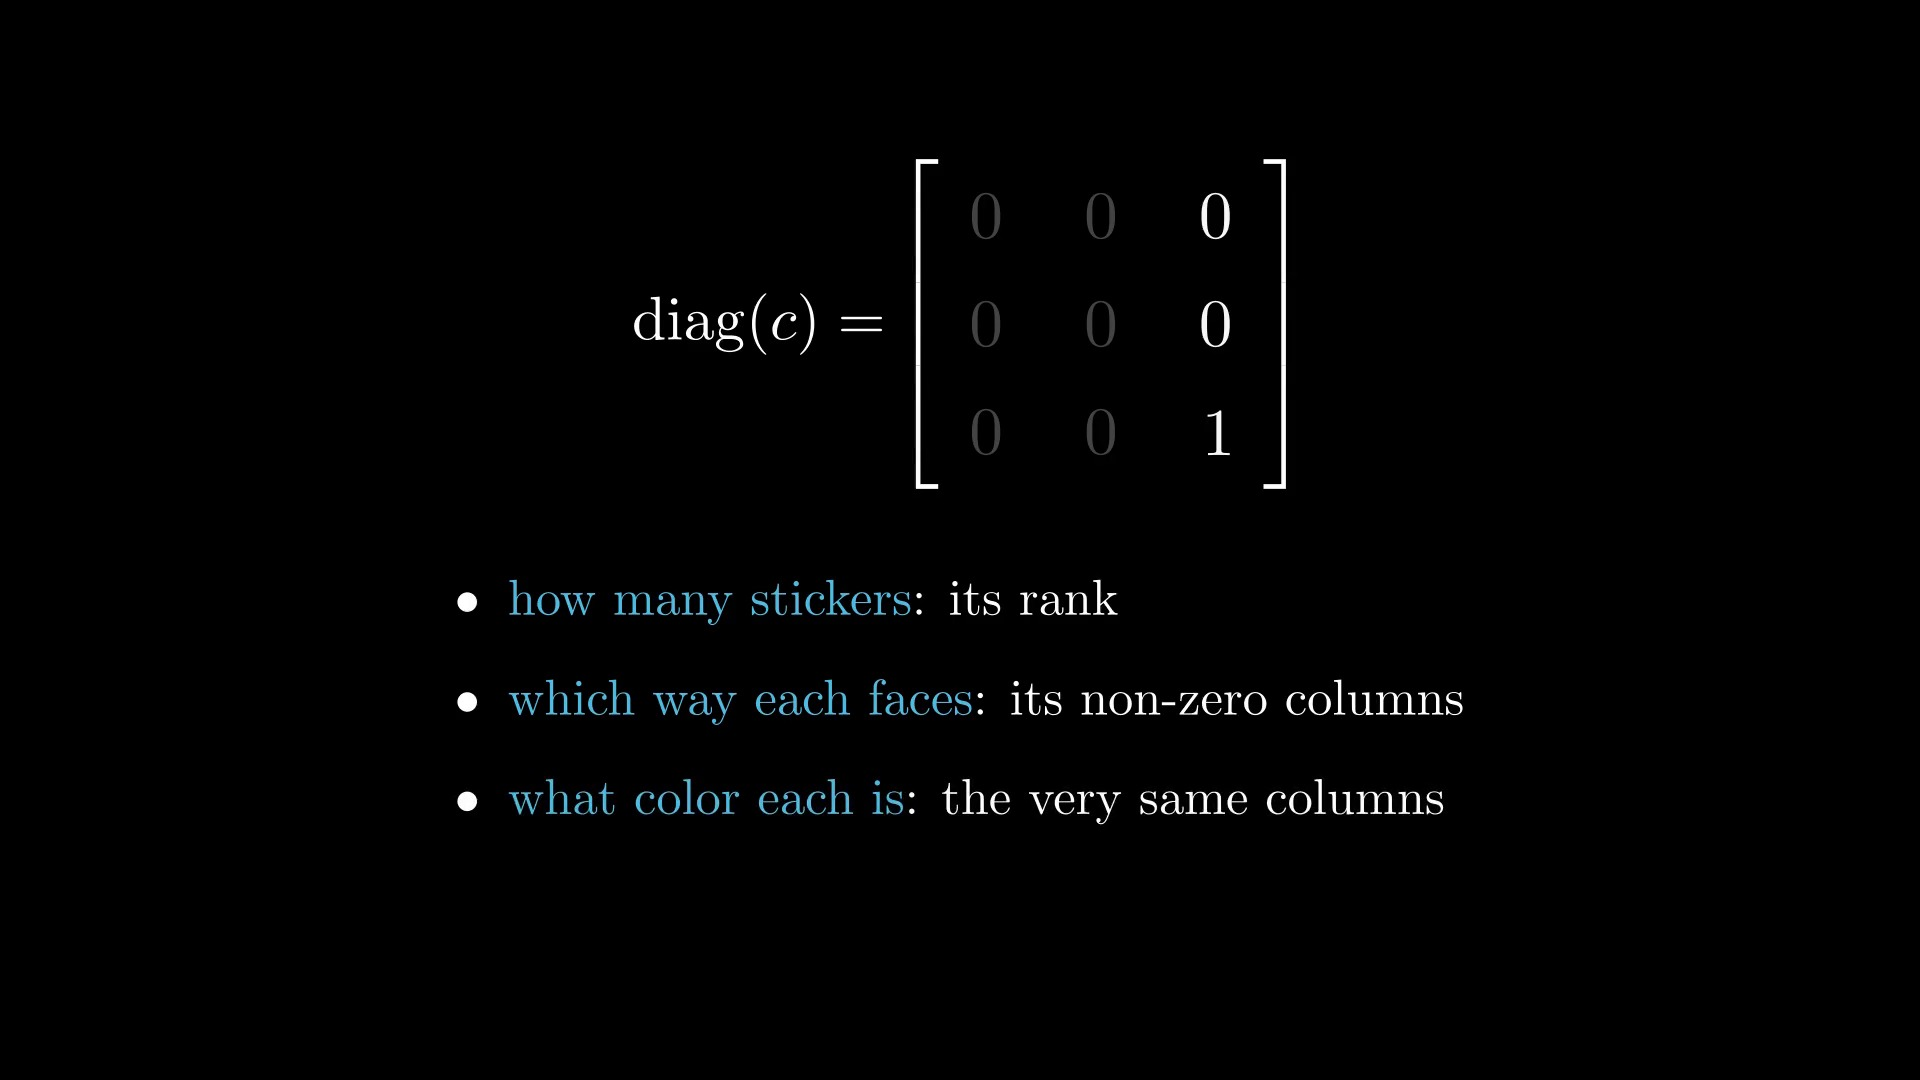
\includegraphics[width=0.90\textwidth]{figures/fig_14_diag_c_meaning.jpg}
\caption{同一个 $\mathrm{diag}(c)$ 给出贴纸的数量、朝向与颜色\vtag}
\label{fig:meaning}
\end{figure}
\srcnote{00:08:26--00:08:44}
\end{minipage}

\subsection{本章小结}

颜色不必另建标签，它就是 $\pm\mathbf{e}_x,\pm\mathbf{e}_y,\pm\mathbf{e}_z$。对单个小立方块，$\mathrm{diag}(c)$ 的列把贴纸的朝向和颜色写成同一组向量，零列则自动表示“这个方向没有贴纸”。打乱之后，这些列还要跟着块一起转，这就是下一节的配置 $(c,R)$。

\section{状态只需一对 $(c,R)$：位置与贴纸如何旋转}

打乱开始以后，小立方块会被带到魔方的其他位置。但它是一整块固体，能做的只有整体移动和整体转动，而且每次走法都是绕原点旋转。根据前面的规则，绕原点的旋转是一个矩阵；接连多次转动仍然是一次旋转。因此，无论这块是怎么走到现在这个取向的，它当前的取向都可以写成一个旋转矩阵 $R$。

完整的描述是一对配置 $(c,R)$：$c$ 用家乡地址命名这块，$R$ 记下它已经被转过的取向。在复原的魔方上，每一块的 $R$ 都是单位阵，也就是还没有转过。

现在转动顶面。对讲者一直跟踪的那个角块，$R$ 变成一次四分之一转
\[
R=\begin{bmatrix}0&1&0\\-1&0&0\\0&0&1\end{bmatrix}.
\]
它现在在哪里？把家乡地址旋转一次，也就是把矩阵 $R$ 作用在 $c$ 上，得到位置
\[
p=Rc
=\begin{bmatrix}0&1&0\\-1&0&0\\0&0&1\end{bmatrix}
\begin{bmatrix}1\\1\\1\end{bmatrix}
=\begin{bmatrix}1\\-1\\1\end{bmatrix}.
\]
\begin{itemize}
\item $c=(1,1,1)$ 是家乡地址（前、右、上）。
\item $p=Rc$ 是当前所在位置，算出来是 $(1,-1,1)$，即前、左、上，与画面中角块的去向一致。
\end{itemize}

\noindent\begin{minipage}{\textwidth}
\begin{figure}[H]
\centering
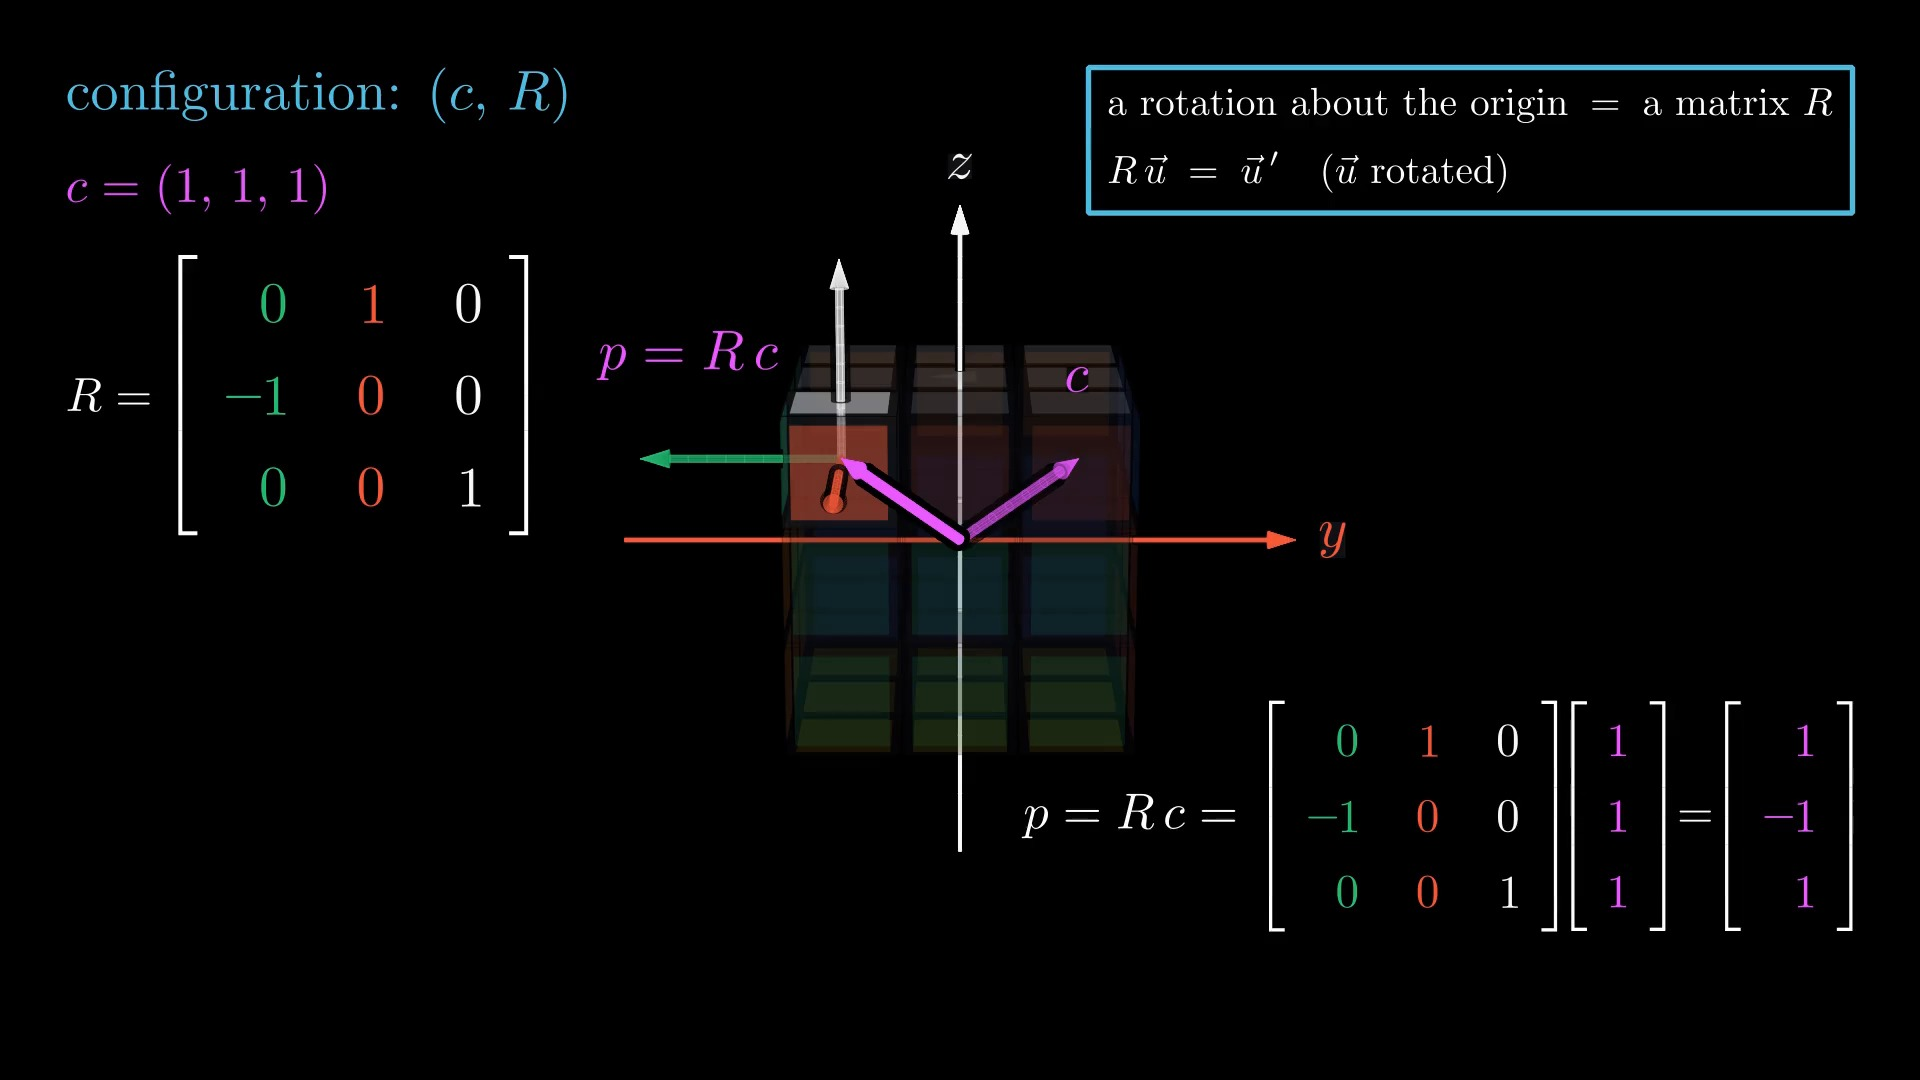
\includegraphics[width=0.90\textwidth]{figures/fig_15_position_Rc.jpg}
\caption{顶面转动后，用 $p=Rc$ 把家乡地址 $(1,1,1)$ 送到 $(1,-1,1)$\vtag}
\label{fig:pRc}
\end{figure}
\srcnote{00:09:38--00:09:55}
\end{minipage}

贴纸指向哪里？同样把 $R$ 作用在 $\mathrm{diag}(c)$ 上。矩阵乘法按列进行，于是一次就旋转了全部贴纸。画面中，绿色改指向左，红色改指向前。

\noindent\begin{minipage}{\textwidth}
\begin{figure}[H]
\centering
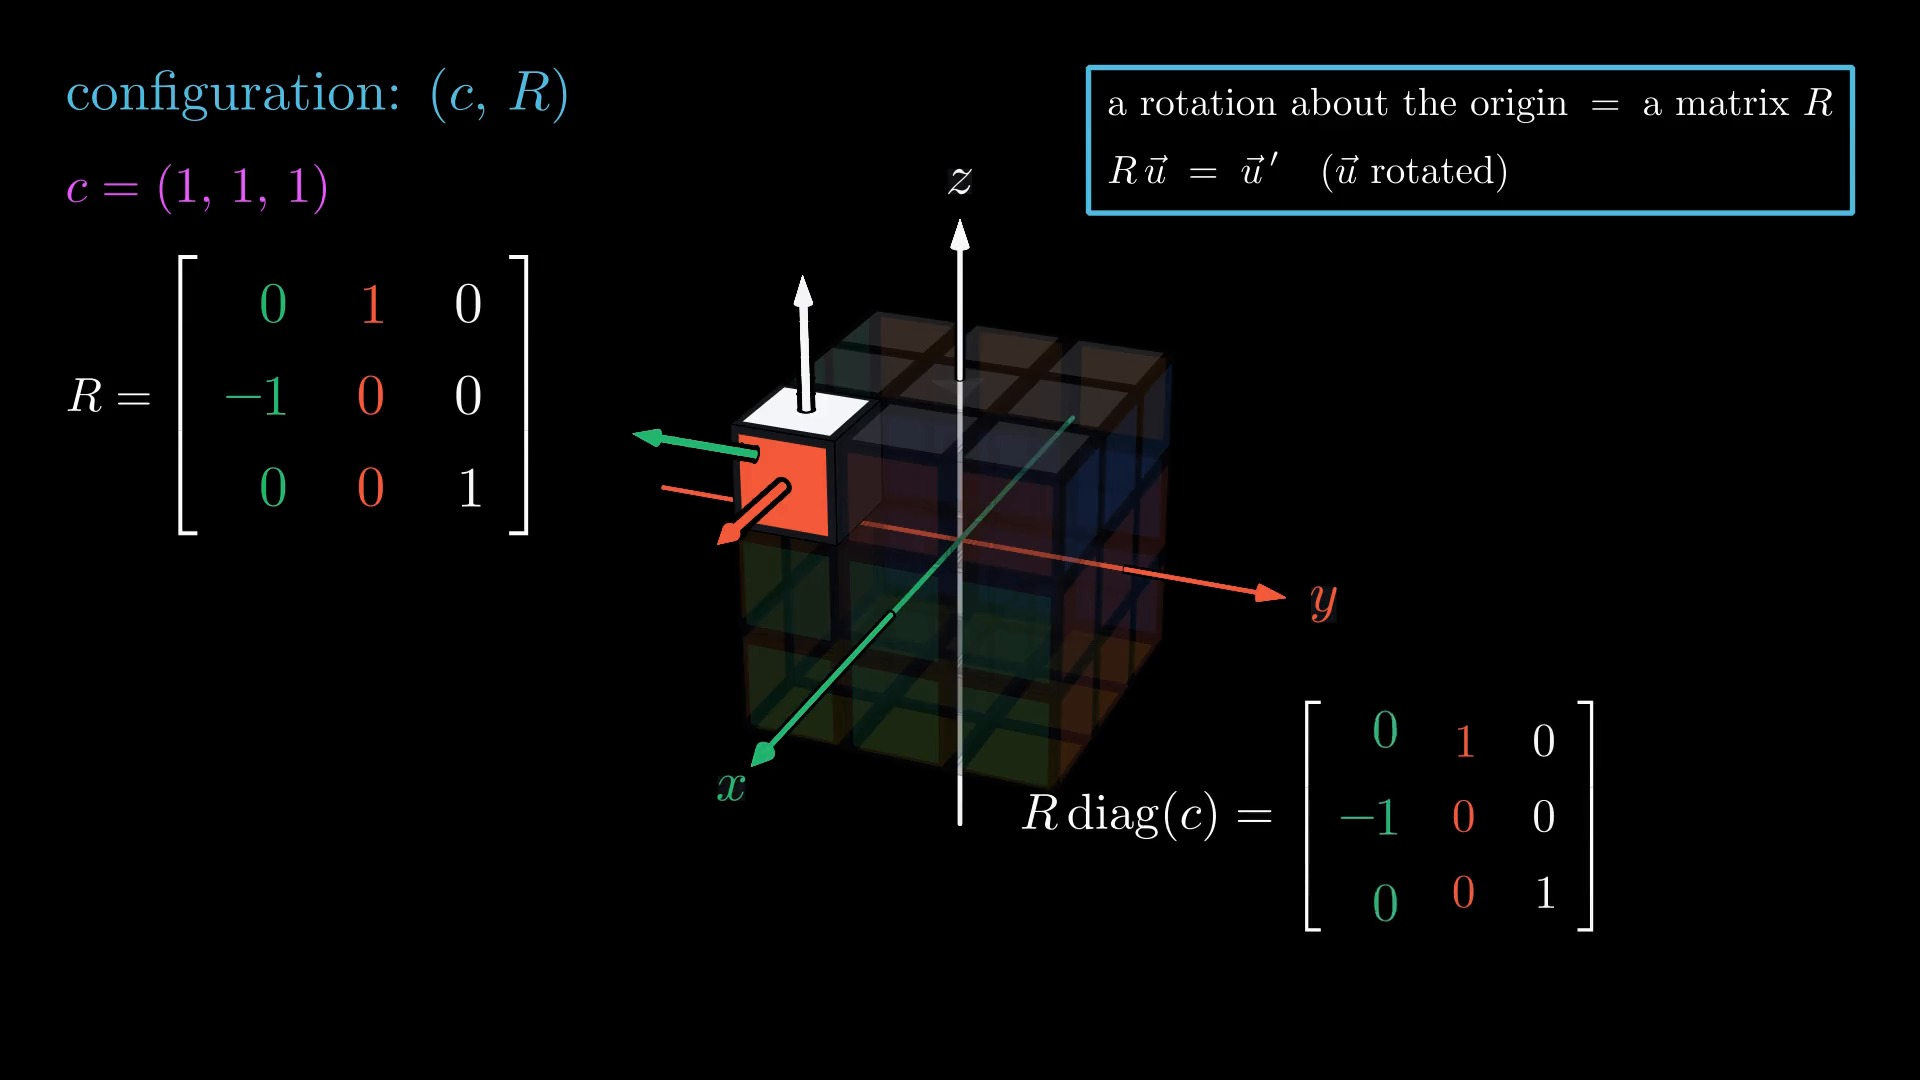
\includegraphics[width=0.90\textwidth]{figures/fig_16_sticker_Rdiag.jpg}
\caption{贴纸朝向由 $R\,\mathrm{diag}(c)$ 给出；对这一角块，$\mathrm{diag}(c)$ 是单位阵，故结果就是 $R$ 本身\vtag}
\label{fig:Rdiag}
\end{figure}
\srcnote{00:09:55--00:10:10}
\end{minipage}

再转前面。角块回到了家乡：$Rc=c$。可是贴纸已经扭转——绿色朝上，而不再朝前。于是 $R$ 作用在 $\mathrm{diag}(c)$ 上，得不到原来的 $\mathrm{diag}(c)$。位置对了，并不等于复原。

\noindent\begin{minipage}{\textwidth}
\begin{figure}[H]
\centering
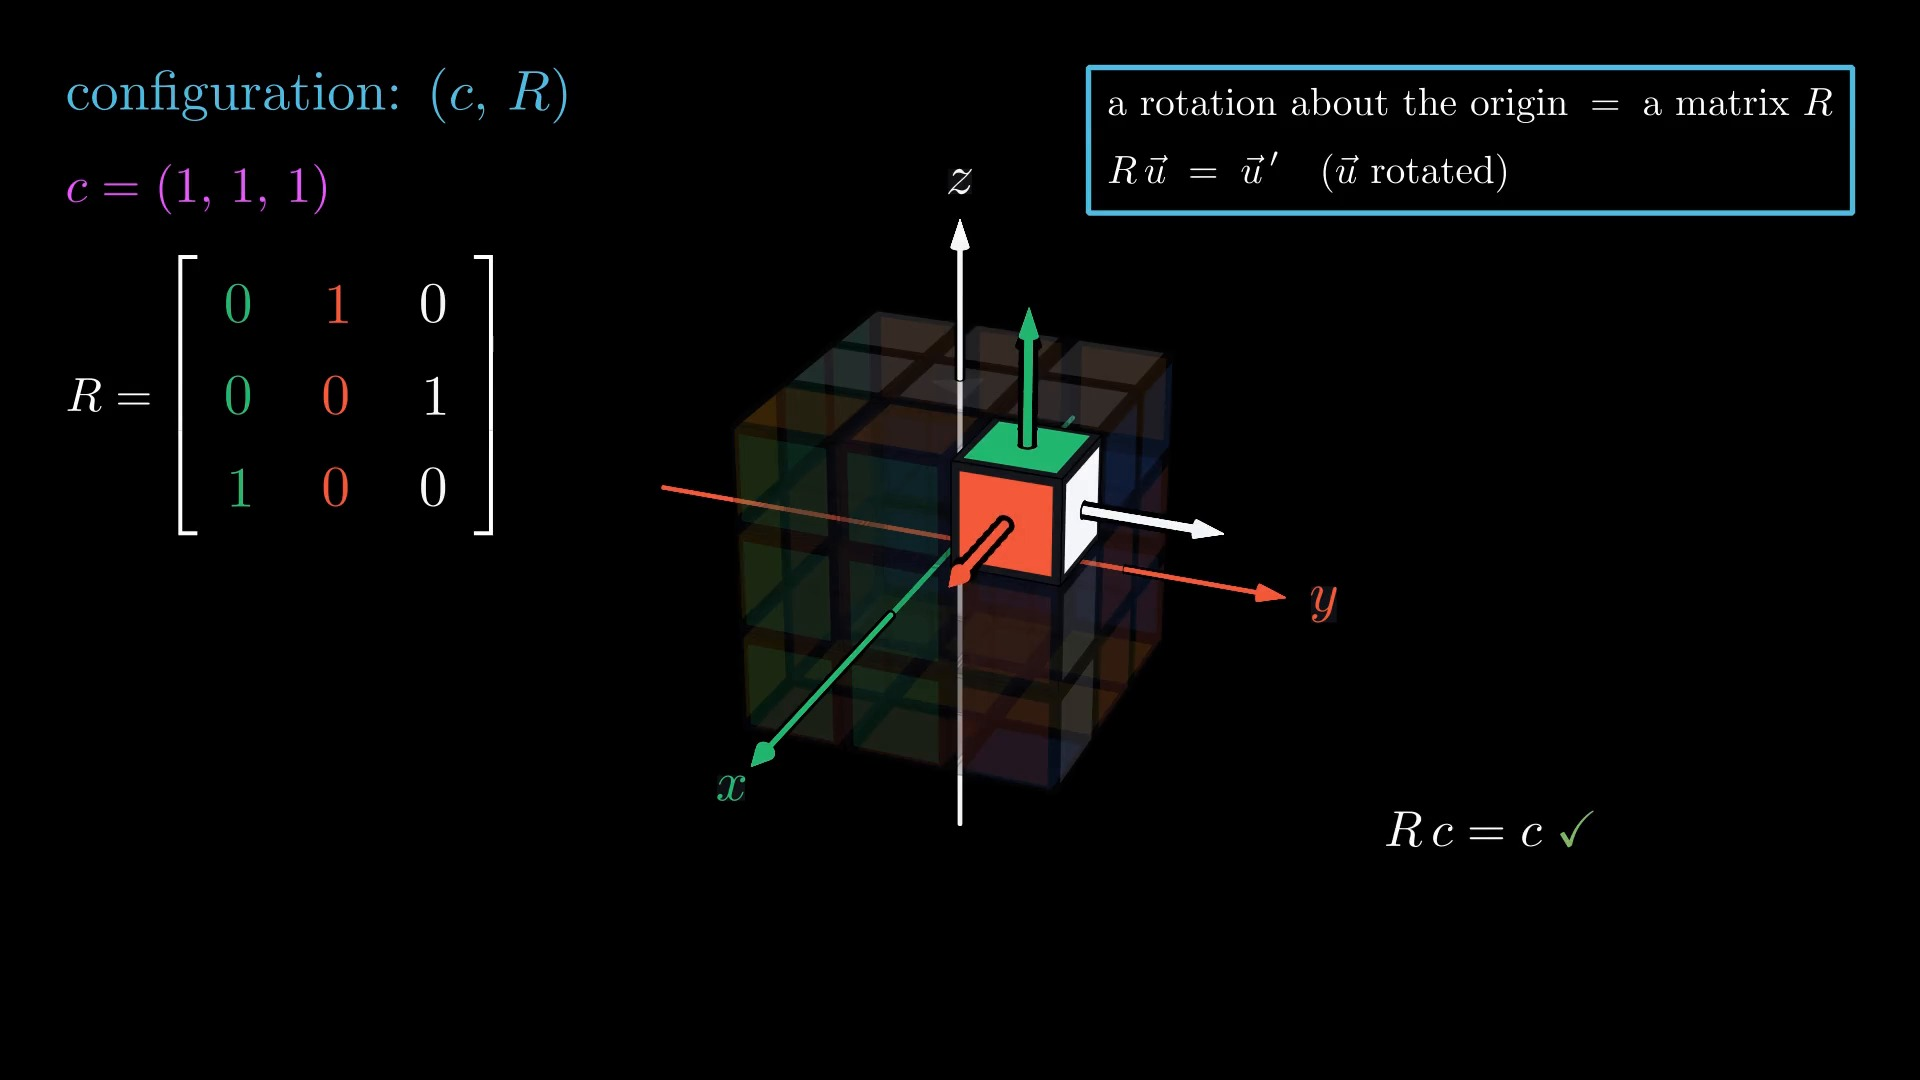
\includegraphics[width=0.90\textwidth]{figures/fig_17_twisted_corner.jpg}
\caption{角块已回家乡（$Rc=c$），但贴纸发生扭转，绿色指向上方\vtag}
\label{fig:twist}
\end{figure}
\srcnote{00:10:10--00:10:25}
\end{minipage}

\begin{warningbox}{位置正确不等于已经复原}
$Rc=c$ 只说明这块回到了家乡槽位。若 $R\,\mathrm{diag}(c)\neq\mathrm{diag}(c)$，贴纸仍是拧过的。后文的复原判定必须同时看取向，而不能只看位置。
\end{warningbox}

讲者的结论是：整个魔方的状态，就是每个小立方块一个配置。不需要贴纸列表，也不需要为扭转的角或翻转的棱另设标志。

\subsection{本章小结}

一对 $(c,R)$ 就写完一个小立方块：位置是 $p=Rc$，贴纸朝向是 $R\,\mathrm{diag}(c)$。下一步要回答，一次具体的面旋转，怎样选出该转的那些块，又怎样更新它们的 $R$。

\section{一步转动：点积筛选，矩阵相乘}

以转动顶面为例。被带动的是顶层里 $z=1$ 的那些小立方块。要写成对任意一面都适用的法则，先取该面的轴向量 $\mathbf{v}$；顶面的 $\mathbf{v}$ 就是指向上的 $\mathbf{e}_z$。再把 $\mathbf{v}$ 与每块当前的位置 $p$ 做点积。与单位轴做点积，量的是 $p$ 沿这个轴走了多远。讲者再次指向 \emph{Essence of Linear Algebra} 中关于点积与对偶的一章，并给出直接算法：把对应坐标相乘再相加。对 $\mathbf{v}=\mathbf{e}_z=(0,0,1)$，
\[
\mathbf{v}\cdot p=(0,0,1)\cdot(x,y,z)=0\cdot x+0\cdot y+1\cdot z=z.
\]
\begin{itemize}
\item $\mathbf{v}$：该面的轴，这里是 $\mathbf{e}_z$。
\item $p=(x,y,z)$：小立方块的当前位置。
\item 结果就是高度 $z$：顶层为 $+1$，中层为 $0$，底层为 $-1$。
\end{itemize}
因此顶层恰好是 $\mathbf{v}\cdot p>0$ 的那些块。又因为 $p=Rc$，判别写成
\[
\mathbf{v}\cdot(Rc)>0.
\]
每个小立方块做一次点积，该层就自己选出来了。因为用的是当前的位置 $p=Rc$，一块先前被转到顶层之后，下一次转顶面时仍会被同一条不等式选中；不必维护一张“谁在顶层”的名单。

\noindent\begin{minipage}{\textwidth}
\begin{figure}[H]
\centering
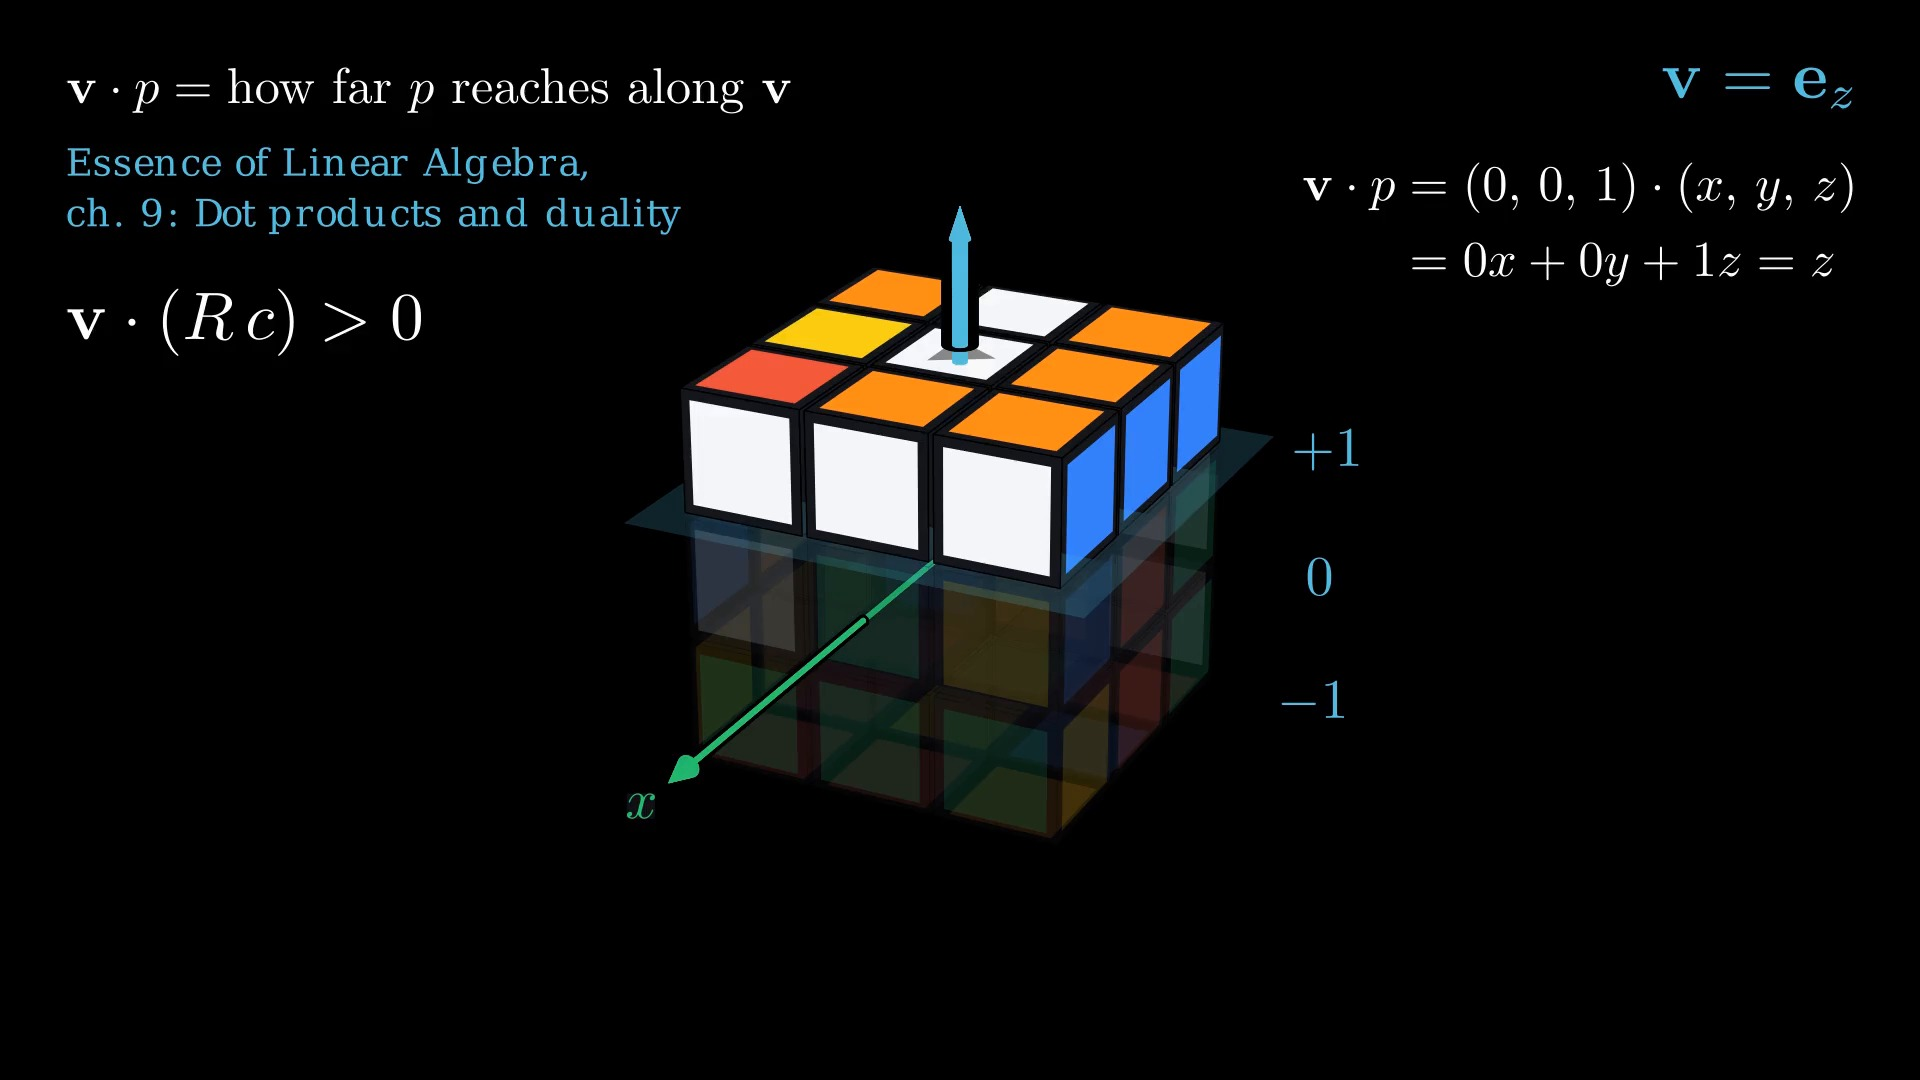
\includegraphics[width=0.90\textwidth]{figures/fig_18_layer_select.jpg}
\caption{用 $\mathbf{v}=\mathbf{e}_z$ 的点积量出高度：$z=+1,0,-1$ 对应上、中、下；顶层满足 $\mathbf{v}\cdot(Rc)>0$\vtag}
\label{fig:dot}
\end{figure}
\srcnote{00:11:18--00:11:37}
\end{minipage}

转动本身是一次四分之一旋转，记为矩阵 $M$。写法仍用回顾里的技巧：看三个基向量落到哪里，那就是 $M$ 的列。讲者给出：$\mathbf{e}_x$ 落到 $-\mathbf{e}_y$，即 $(0,-1,0)$；$\mathbf{e}_y$ 落到 $\mathbf{e}_x$，即 $(1,0,0)$；$\mathbf{e}_z$ 留在原地，即 $(0,0,1)$。最后这一条再次是转动轴，也就是特征向量。于是
\[
M=\begin{bmatrix}0&1&0\\-1&0&0\\0&0&1\end{bmatrix}.
\]
\begin{itemize}
\item 第一列是 $\mathbf{e}_x$ 的落点 $(0,-1,0)$。
\item 第二列是 $\mathbf{e}_y$ 的落点 $(1,0,0)$。
\item 第三列是转轴 $\mathbf{e}_z$，仍为 $(0,0,1)$。
\end{itemize}
每一个被选中的小立方块都把自己的 $R$ 左乘上 $M$：
\[
R\leftarrow MR.
\]
这就是整步走法：一次点积用来筛选，一次矩阵乘法用来转动。

\noindent\begin{minipage}{\textwidth}
\begin{figure}[H]
\centering
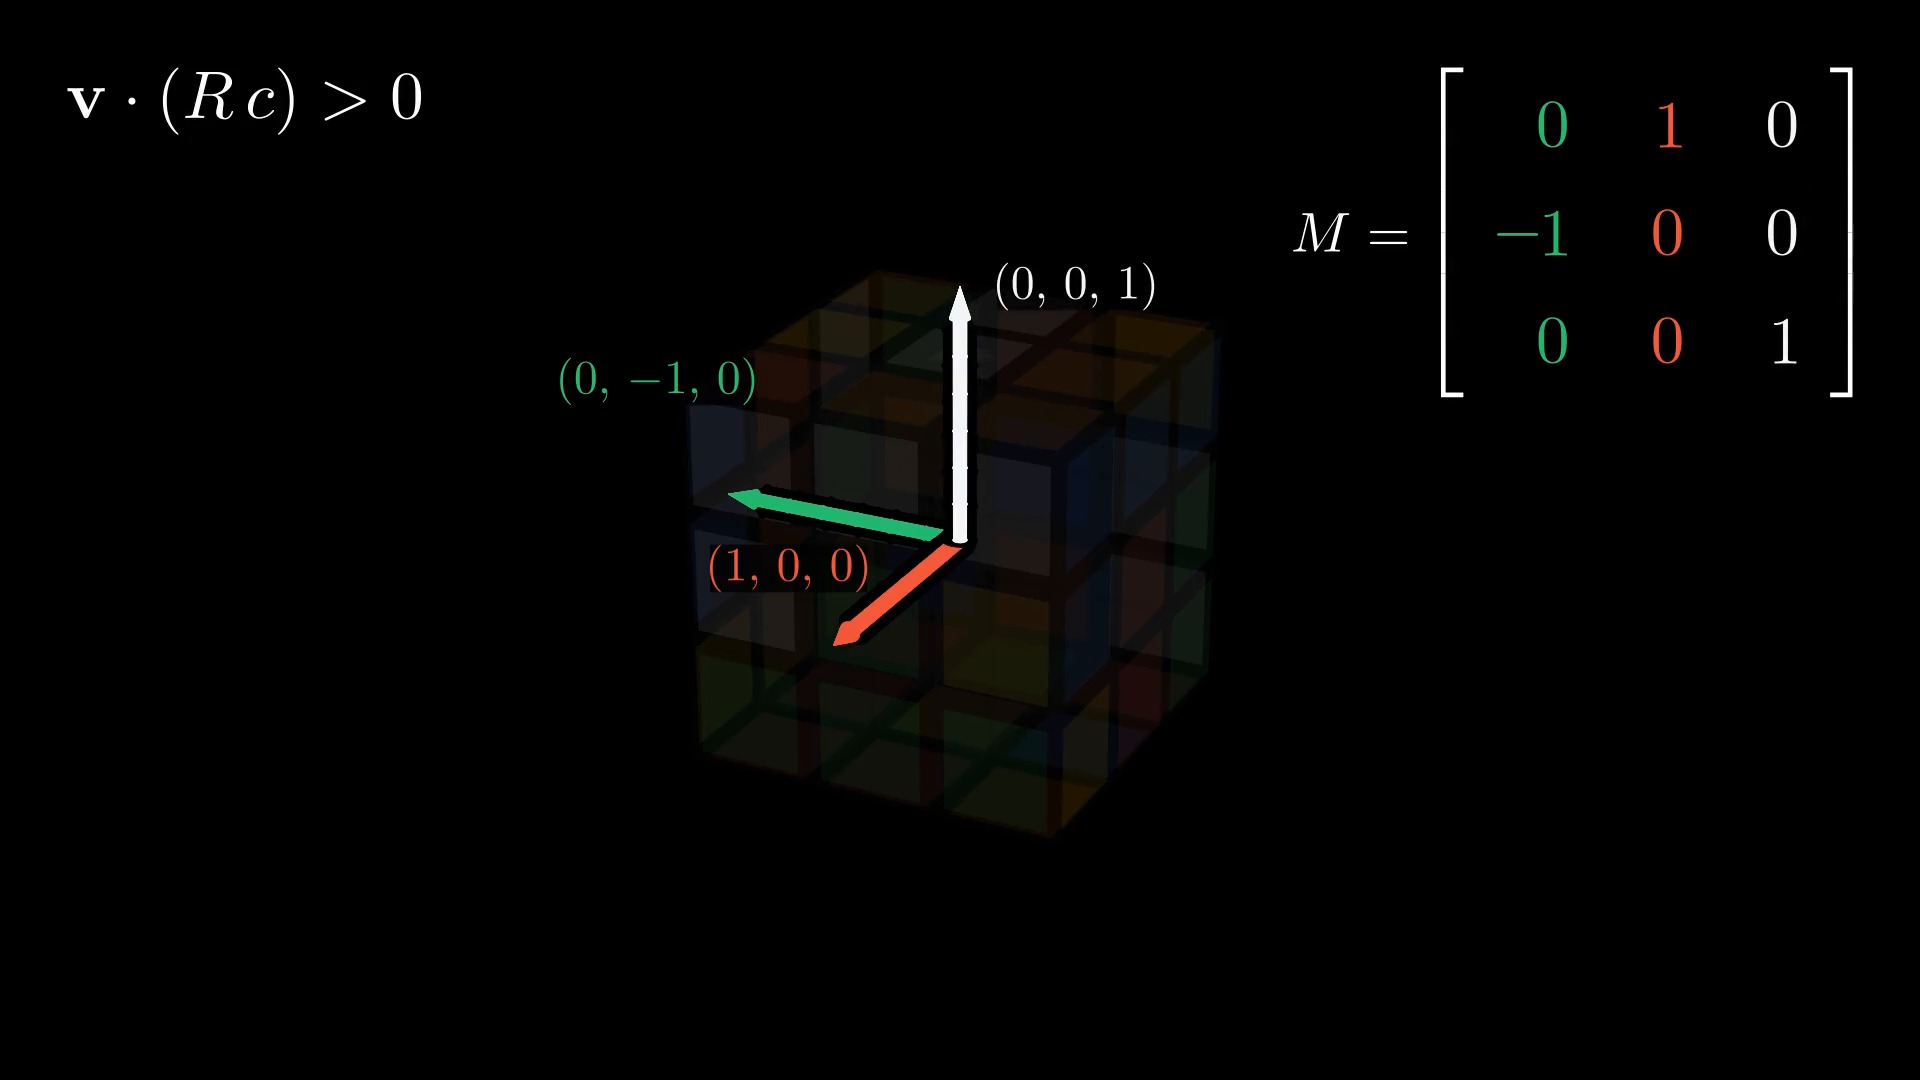
\includegraphics[width=0.90\textwidth]{figures/fig_19_move_matrix_M.jpg}
\caption{顶面四分之一转的矩阵 $M$：三列分别是 $\mathbf{e}_x$、$\mathbf{e}_y$、$\mathbf{e}_z$ 的落点\vtag}
\label{fig:M}
\end{figure}
\srcnote{00:11:45--00:12:13}
\end{minipage}

讲者还指出一个计算上的好处：这些矩阵的条目只有 $0$、$1$ 或 $-1$，无论走多少步，算术都保持精确，不会累积舍入。屏幕上的实现与数学一一对应，整段走法逻辑就是下面这几行。

\noindent\begin{minipage}{\textwidth}
\begin{figure}[H]
\centering
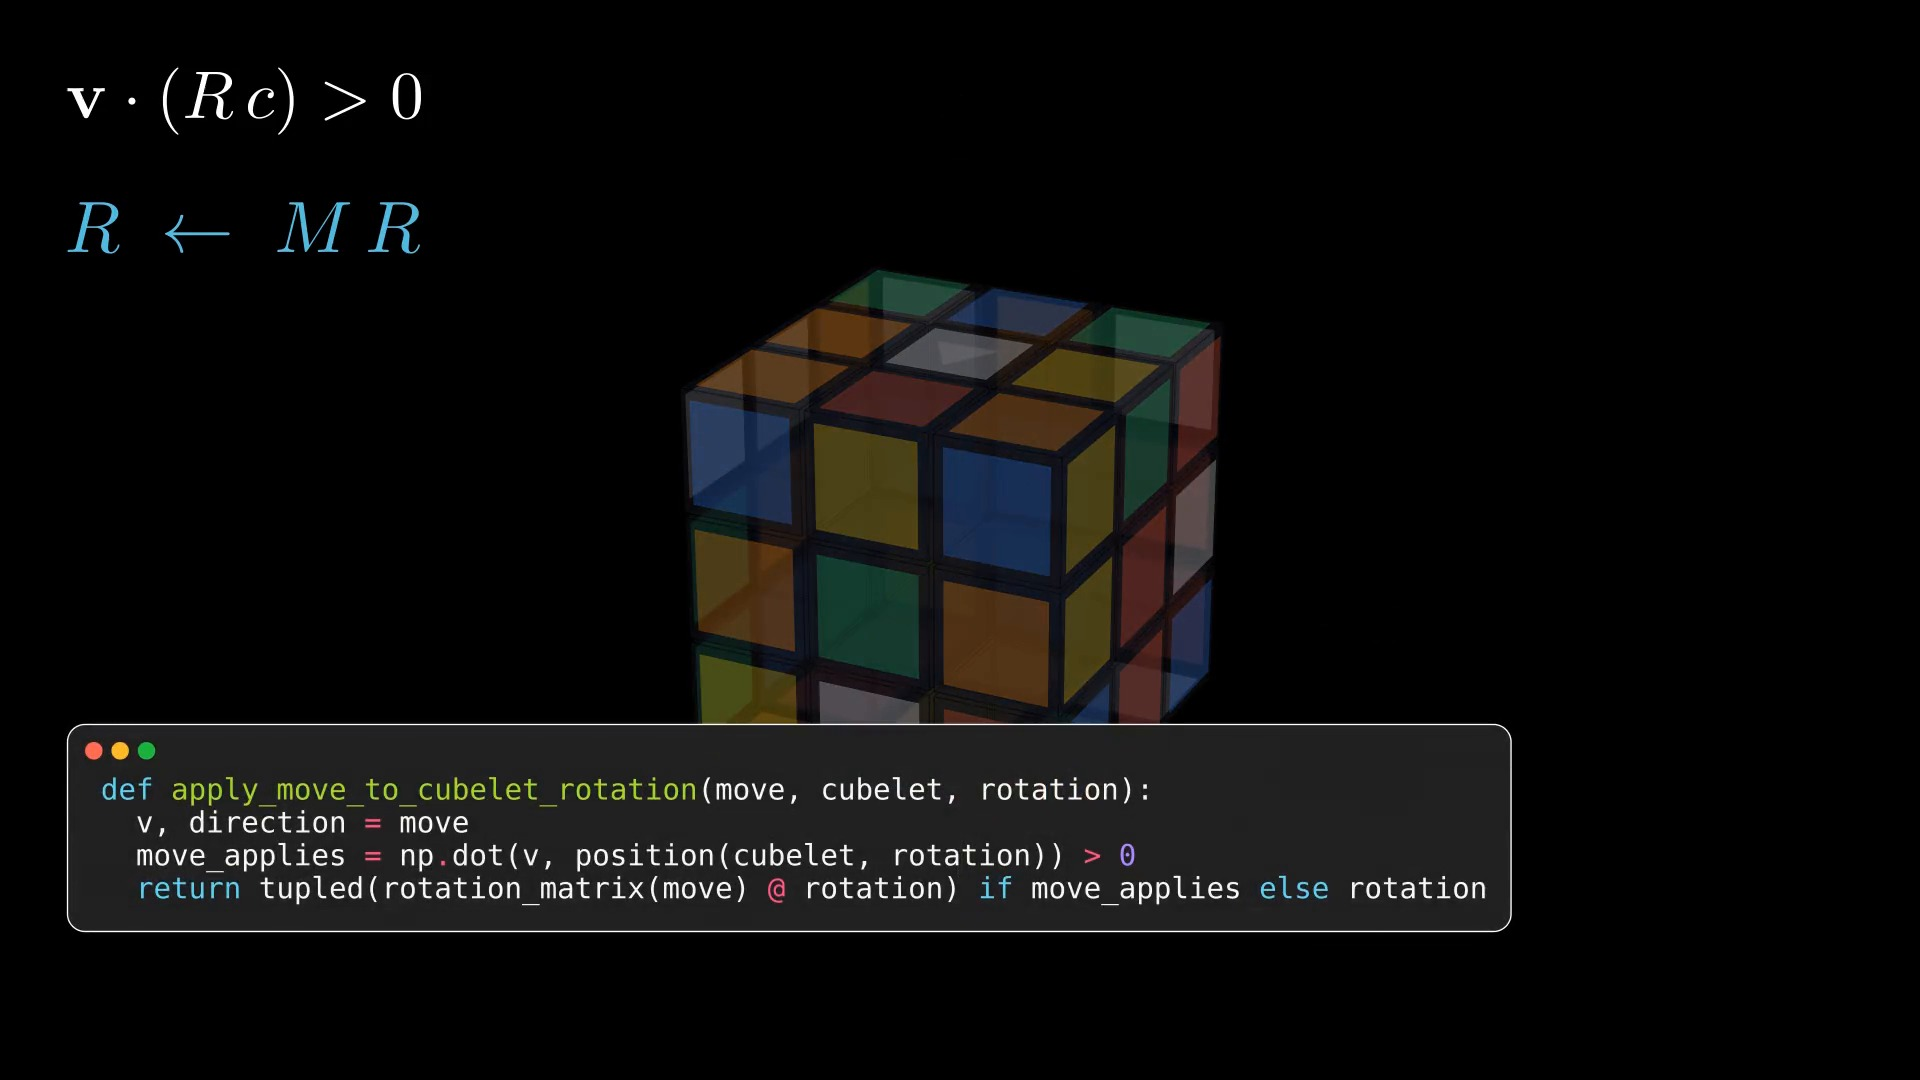
\includegraphics[width=0.90\textwidth]{figures/fig_20_move_code.jpg}
\caption{走法在代码中的全部逻辑：用点积判断是否在该层，再用矩阵乘法更新取向\vtag}
\label{fig:code}
\end{figure}
\srcnote{00:12:28--00:12:36}
\end{minipage}

\begin{lstlisting}[caption={视频中展示的走法函数：点积筛选，矩阵更新取向},basicstyle=\ttfamily\footnotesize,breaklines=true]
def apply_move_to_cubelet_rotation(move, cubelet, rotation):
    v, direction = move
    move_applies = np.dot(v, position(cubelet, rotation)) > 0
    return tupled(rotation_matrix(move) @ rotation) if move_applies else rotation
\end{lstlisting}

\begin{importantbox}{一步走法的两句总结}
一次点积决定这块是否在被转的那一层；一次矩阵乘法 $R\leftarrow MR$ 执行转动。二者合起来就是全部走法逻辑。
\end{importantbox}

\subsection{本章小结}

选层不靠枚举槽位，而靠 $\mathbf{v}\cdot(Rc)>0$；转动不靠置换表，而靠把基的落点写成 $M$ 再左乘。余下的最后一个问题是：什么时候可以宣布魔方已经复原？

\section{何时复原：$R\,\mathrm{diag}(c)=\mathrm{diag}(c)$}

一个小立方块算作复原，当且仅当它的每一张贴纸都朝着与自己颜色相同的那个中心。写成符号，就是把 $R$ 作用在 $\mathrm{diag}(c)$ 上，应当原样得到 $\mathrm{diag}(c)$：
\[
R\,\mathrm{diag}(c)=\mathrm{diag}(c).
\]
\begin{itemize}
\item 左侧是当前取向作用在家乡贴纸矩阵上。
\item 右侧是尚未扭转的家乡贴纸。相等意味着每张贴纸都对着同色中心。
\end{itemize}
前面那个扭转的角块，位置是对的（$Rc=c$），但贴纸不对，这个检验会把它抓住。下图则给出通过检验的情形：绿色朝前、红色朝右、白色朝上，与三个中心一致。

\noindent\begin{minipage}{\textwidth}
\begin{figure}[H]
\centering
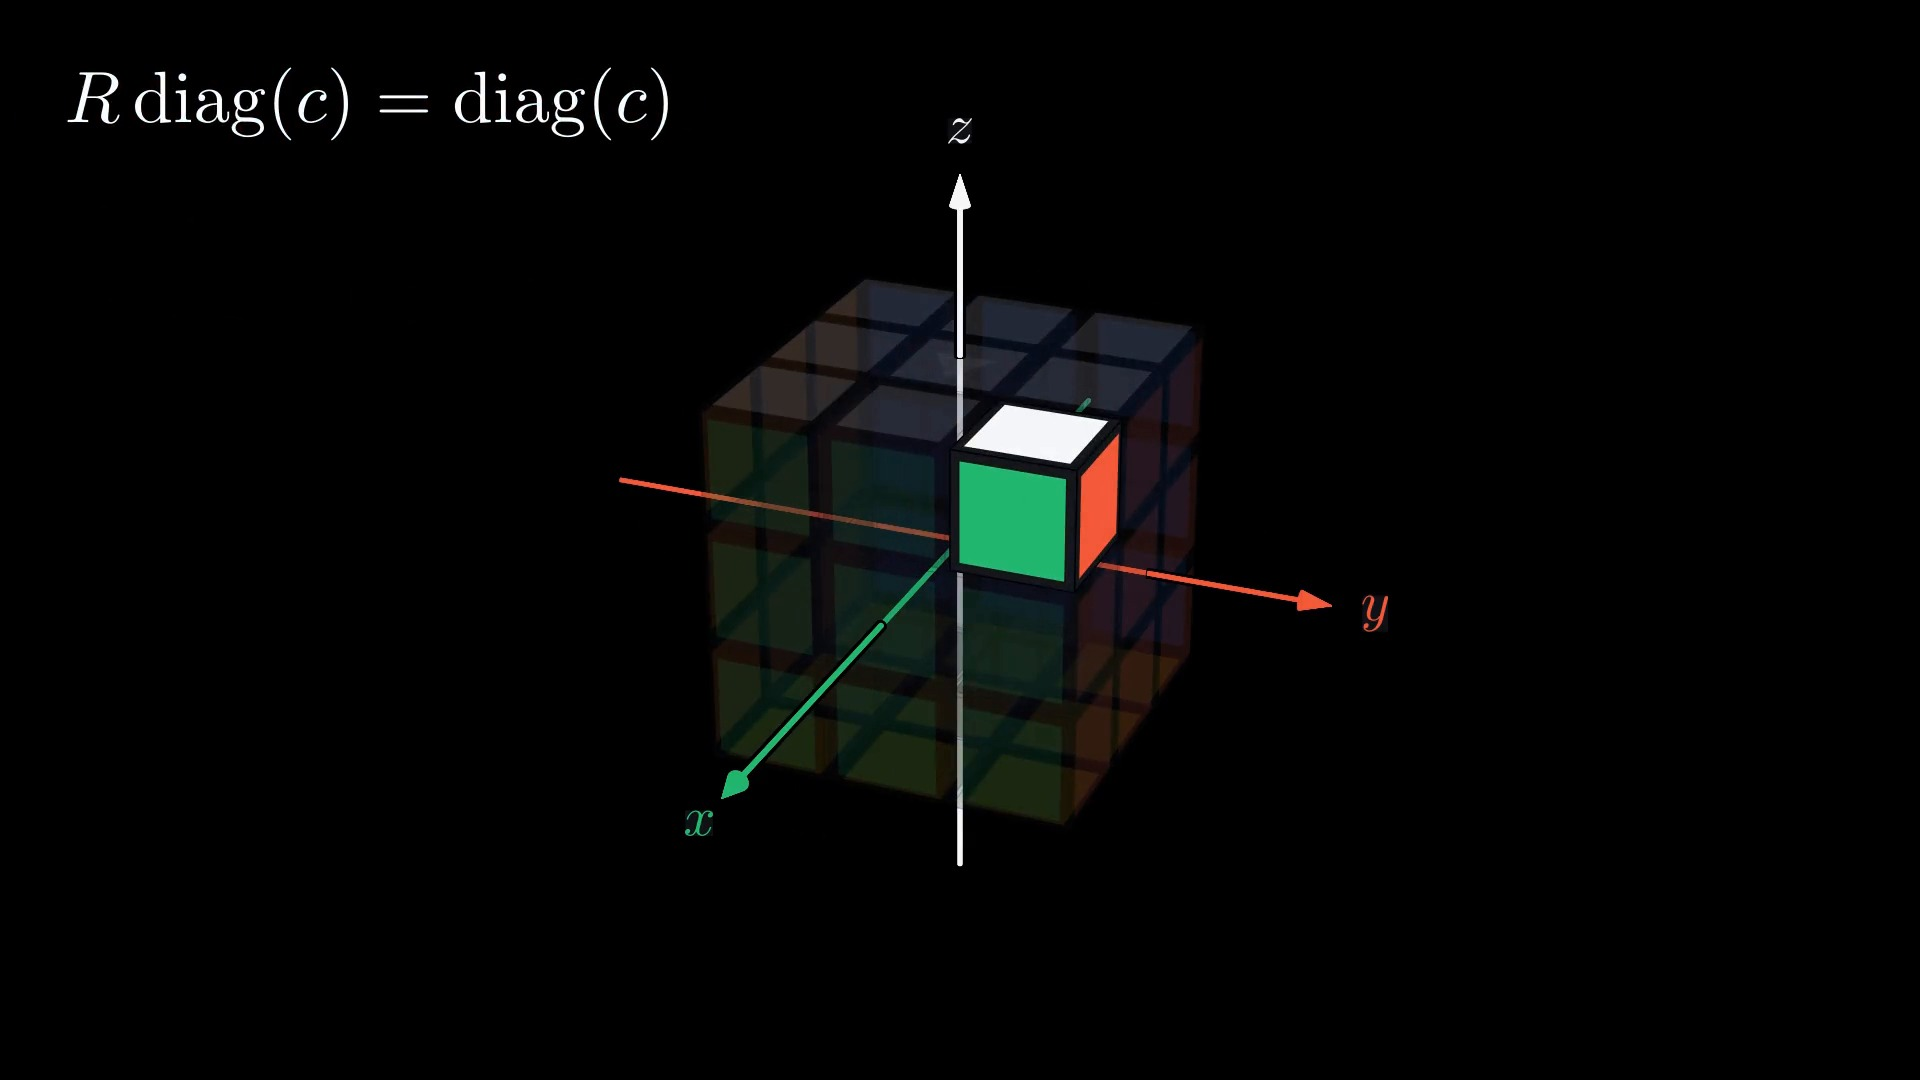
\includegraphics[width=0.90\textwidth]{figures/fig_21_solved_test.jpg}
\caption{复原条件 $R\,\mathrm{diag}(c)=\mathrm{diag}(c)$：角块的三张贴纸分别对着绿、红、白三个中心\vtag}
\label{fig:solved}
\end{figure}
\srcnote{00:12:39--00:13:00}
\end{minipage}

这里有一个细致之处。对一个角块，三张贴纸都朝向家乡，会迫使 $R$ 只能是单位阵；对一条棱，两个方向被钉死，旋转也没有剩下的自由度。中心却只有一张贴纸。讲者在白色中心上画了一个小标记，好让人看清它在转：此时 $R$ 是一次四分之一转，并不是单位阵。但把它作用到 $\mathrm{diag}(c)$ 上，只有最后一列非零，而这次转动恰好把这一列留在原地，于是仍然得到 $\mathrm{diag}(c)$，检验通过。在普通魔方上，中心的这点自旋本来就看不见，编码也同样不在意。检验的严格程度，正好与颜色所规定的一样。

\noindent\begin{minipage}{\textwidth}
\begin{figure}[H]
\centering
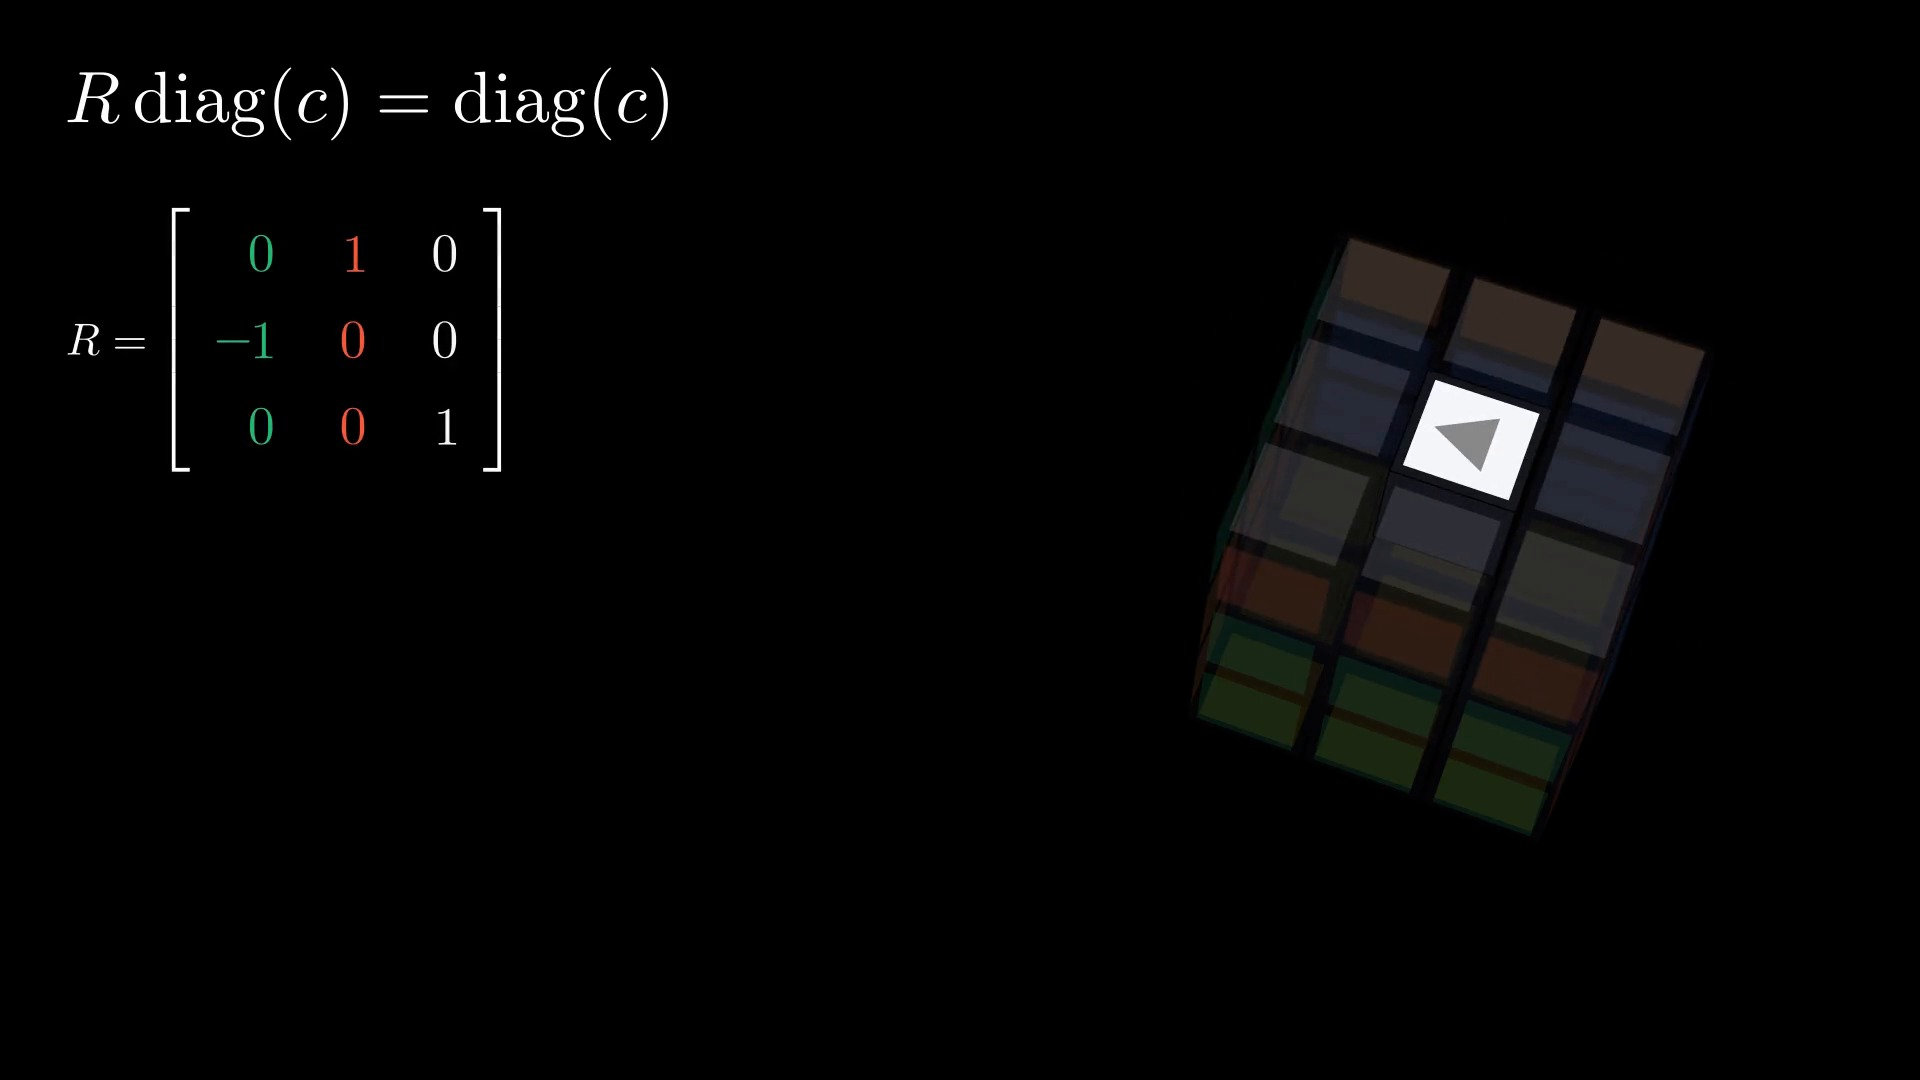
\includegraphics[width=0.90\textwidth]{figures/fig_22_center_spin.jpg}
\caption{中心只有一张贴纸：即使 $R$ 是四分之一转，作用在 $\mathrm{diag}(c)$ 上仍保持不变，检验通过。白心上的三角标记用来显示这次自旋\vtag}
\label{fig:center}
\end{figure}
\srcnote{00:13:00--00:13:33}
\end{minipage}

讲者说，代码里整段复原检验只有三行，并且直接来自上述等式。

\begin{warningbox}{中心可以“空转”}
角块和棱块一旦方向对齐，$R$ 就必须是单位阵；中心只有一个非零列，绕自己法向的自旋不会改变 $\mathrm{diag}(c)$。不要把 $R=I$ 误当成对每一种零件都必要的条件。
\end{warningbox}

\subsection{本章小结}

复原不是“每块都回到槽位”，而是 $R\,\mathrm{diag}(c)=\mathrm{diag}(c)$：贴纸与同色中心同向。这个条件对扭转的角块足够严格，对中心的不可见自旋又恰好足够宽松。至此，表示、走法与判定都已经闭合。

\section{总结与延伸}

讲者在收束时把整套模型压成几行，与下图一一对应：

\noindent\begin{minipage}{\textwidth}
\begin{figure}[H]
\centering
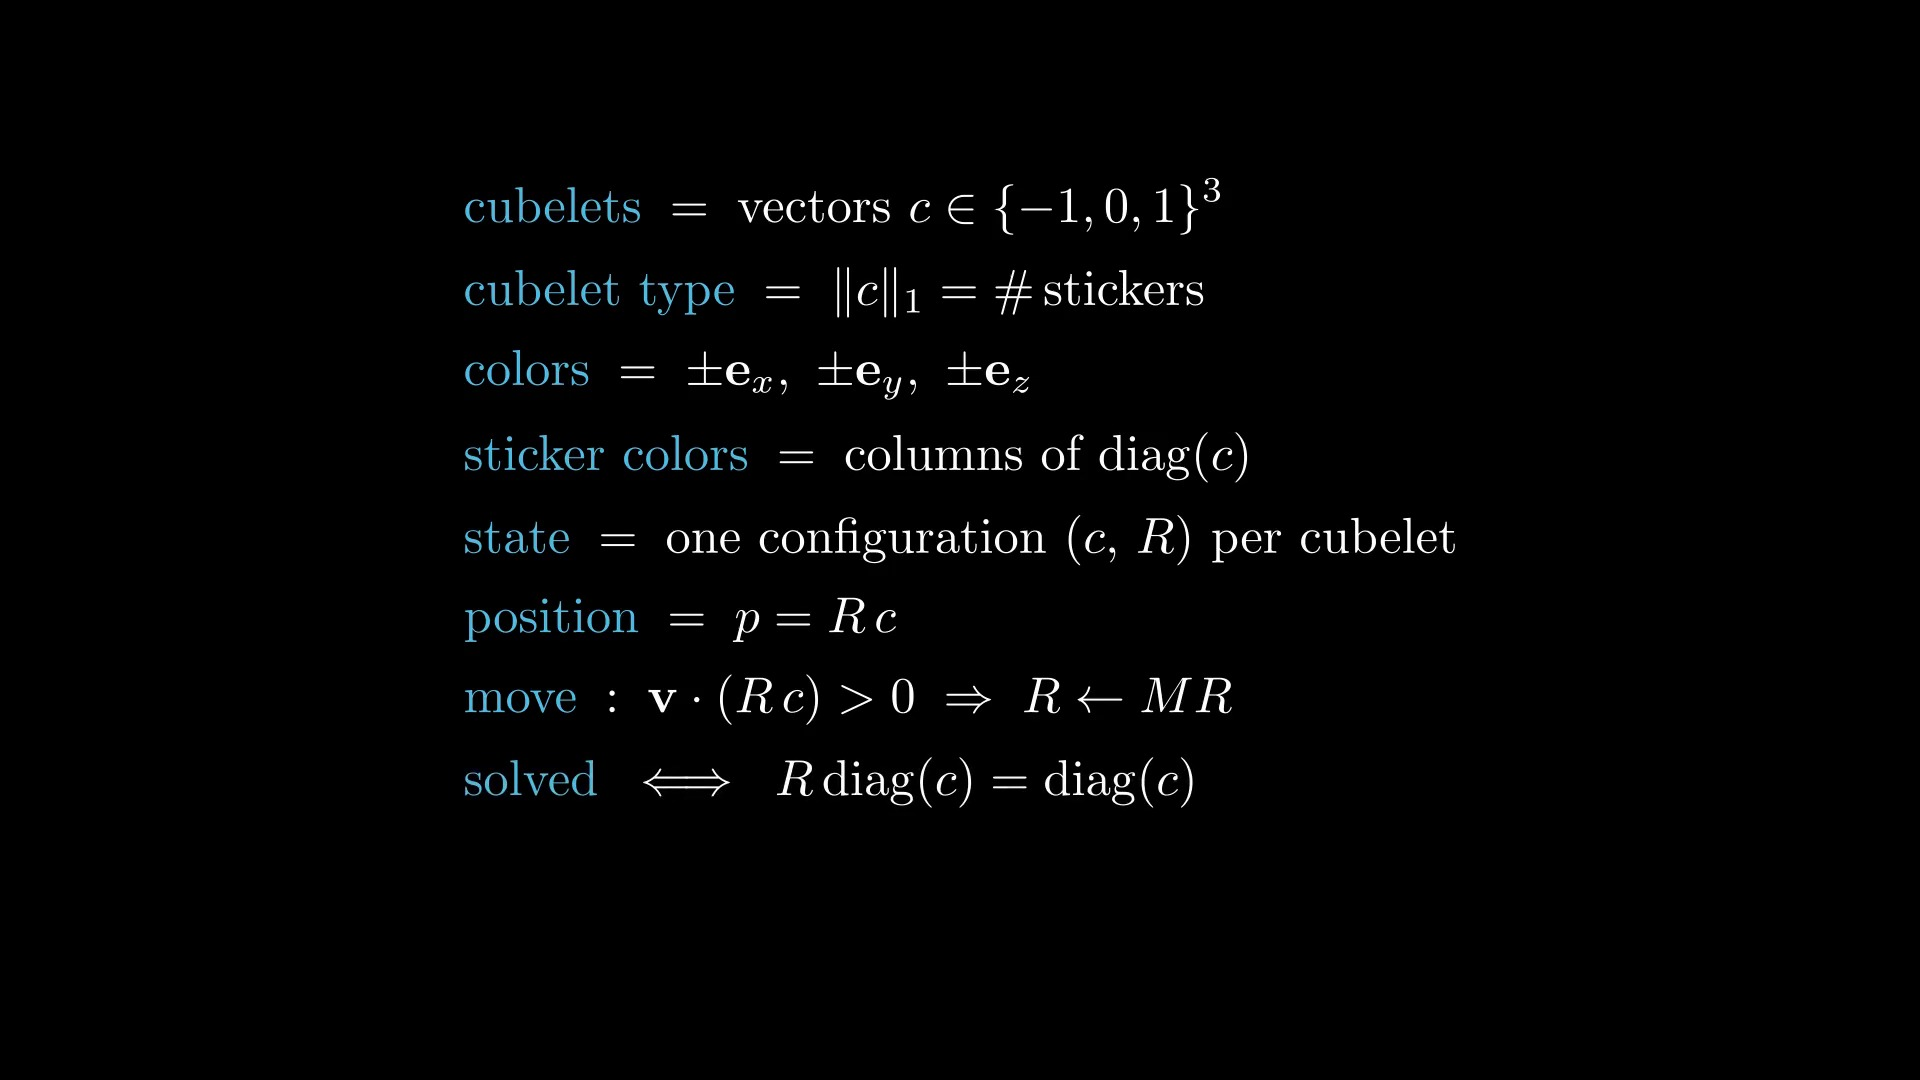
\includegraphics[width=0.90\textwidth]{figures/fig_23_model_summary.jpg}
\caption{讲者给出的模型总结：从地址向量到复原判定\vtag}
\label{fig:sum}
\end{figure}
\srcnote{00:13:48--00:14:35}
\end{minipage}

\begin{itemize}
\item 小立方块是向量 $c\in\{-1,0,1\}^3$。
\item 类型由曼哈顿范数 $\|c\|_1$ 给出，也就是贴纸数。
\item 颜色是 $\pm\mathbf{e}_x,\pm\mathbf{e}_y,\pm\mathbf{e}_z$。
\item 贴纸颜色是 $\mathrm{diag}(c)$ 的列。
\item 状态是每个小立方块一个配置 $(c,R)$。
\item 当前位置是 $p=Rc$。
\item 走法：若 $\mathbf{v}\cdot(Rc)>0$，则 $R\leftarrow MR$。
\item 复原当且仅当 $R\,\mathrm{diag}(c)=\mathrm{diag}(c)$。
\end{itemize}

讲者的原话是：这就是全部模型，其余的东西都从几何里长出来。在这套表示之上，Eigencube 按层求解：用 A-star 搜索，启发函数是每个小立方块离家乡还差多少个四分之一转，最后再加一段经典公式收尾。视频末尾演示了它还原一次打乱，但没有再展开启发式或那串公式的细节。

若这套看法让人觉得亲切，讲者把功劳归于 \emph{Essence of Linear Algebra}，并建议去看那个系列：看过之后，会开始在各处把矩阵看成运动，哪怕是在 1974 年的这件玩具里面。它从来不是一份 54 种颜色的清单，而一直是线性代数。

本讲义把讲者的论证压缩为一条可以用手算核对的路径：先拒绝贴纸列表，再用固定十字建立坐标，让范数、颜色与 $\mathrm{diag}(c)$ 承担分类和贴纸编码，最后用一对 $(c,R)$ 同时写出位置、走法与复原。它的边界也很清楚：视频展示了表示与一步走法的完整数学，以及求解器的层间策略和启发式的一句话描述，但没有在屏幕上推导 A-star 的权值，也没有写出收尾用的那串经典公式。若要继续，自然的下一个问题是：在这套 $(c,R)$ 表示下，那一格启发函数如何写成可计算的四分之一转距离，以及层间衔接时需要哪一段固定公式。

%% --- 正文内容结束 --- %%

\end{document}
